\documentclass[]{article}
\usepackage{lmodern}
\usepackage{amssymb,amsmath}
\usepackage{ifxetex,ifluatex}
\usepackage{fixltx2e} \% provides \textsubscript
\ifnum 0\ifxetex 1\fi\ifluatex 1\fi=0 \% if pdftex
  \usepackage[T1]{fontenc}
  \usepackage[utf8]{inputenc}
\else \% if luatex or xelatex
  \ifxetex
    \usepackage{mathspec}
  \else
    \usepackage{fontspec}
  \fi
  \defaultfontfeatures{Ligatures=TeX,Scale=MatchLowercase}
\fi
\% use upquote if available, for straight quotes in verbatim environments
\IfFileExists{upquote.sty}{\usepackage{upquote}}{}
\% use microtype if available
\IfFileExists{microtype.sty}{\%
\usepackage{microtype}
\UseMicrotypeSet[protrusion]{basicmath} \% disable protrusion for tt fonts
}{}
\usepackage[margin=1in]{geometry}
\usepackage{hyperref}
\hypersetup{unicode=true,
            pdftitle={Assignment4},
            pdfauthor={Kaicheng Luo},
            pdfborder={0 0 0},
            breaklinks=true}
\urlstyle{same}  \% don't use monospace font for urls
\usepackage{color}
\usepackage{fancyvrb}
\newcommand{\VerbBar}{|}
\newcommand{\VERB}{\Verb[commandchars=\\\{\}]}
\DefineVerbatimEnvironment{Highlighting}{Verbatim}{commandchars=\\\{\}}
\% Add ',fontsize=\small' for more characters per line
\usepackage{framed}
\definecolor{shadecolor}{RGB}{248,248,248}
\newenvironment{Shaded}{\begin{snugshade}}{\end{snugshade}}
\newcommand{\KeywordTok}[1]{\textcolor[rgb]{0.13,0.29,0.53}{\textbf{#1}}}
\newcommand{\DataTypeTok}[1]{\textcolor[rgb]{0.13,0.29,0.53}{#1}}
\newcommand{\DecValTok}[1]{\textcolor[rgb]{0.00,0.00,0.81}{#1}}
\newcommand{\BaseNTok}[1]{\textcolor[rgb]{0.00,0.00,0.81}{#1}}
\newcommand{\FloatTok}[1]{\textcolor[rgb]{0.00,0.00,0.81}{#1}}
\newcommand{\ConstantTok}[1]{\textcolor[rgb]{0.00,0.00,0.00}{#1}}
\newcommand{\CharTok}[1]{\textcolor[rgb]{0.31,0.60,0.02}{#1}}
\newcommand{\SpecialCharTok}[1]{\textcolor[rgb]{0.00,0.00,0.00}{#1}}
\newcommand{\StringTok}[1]{\textcolor[rgb]{0.31,0.60,0.02}{#1}}
\newcommand{\VerbatimStringTok}[1]{\textcolor[rgb]{0.31,0.60,0.02}{#1}}
\newcommand{\SpecialStringTok}[1]{\textcolor[rgb]{0.31,0.60,0.02}{#1}}
\newcommand{\ImportTok}[1]{#1}
\newcommand{\CommentTok}[1]{\textcolor[rgb]{0.56,0.35,0.01}{\textit{#1}}}
\newcommand{\DocumentationTok}[1]{\textcolor[rgb]{0.56,0.35,0.01}{\textbf{\textit{#1}}}}
\newcommand{\AnnotationTok}[1]{\textcolor[rgb]{0.56,0.35,0.01}{\textbf{\textit{#1}}}}
\newcommand{\CommentVarTok}[1]{\textcolor[rgb]{0.56,0.35,0.01}{\textbf{\textit{#1}}}}
\newcommand{\OtherTok}[1]{\textcolor[rgb]{0.56,0.35,0.01}{#1}}
\newcommand{\FunctionTok}[1]{\textcolor[rgb]{0.00,0.00,0.00}{#1}}
\newcommand{\VariableTok}[1]{\textcolor[rgb]{0.00,0.00,0.00}{#1}}
\newcommand{\ControlFlowTok}[1]{\textcolor[rgb]{0.13,0.29,0.53}{\textbf{#1}}}
\newcommand{\OperatorTok}[1]{\textcolor[rgb]{0.81,0.36,0.00}{\textbf{#1}}}
\newcommand{\BuiltInTok}[1]{#1}
\newcommand{\ExtensionTok}[1]{#1}
\newcommand{\PreprocessorTok}[1]{\textcolor[rgb]{0.56,0.35,0.01}{\textit{#1}}}
\newcommand{\AttributeTok}[1]{\textcolor[rgb]{0.77,0.63,0.00}{#1}}
\newcommand{\RegionMarkerTok}[1]{#1}
\newcommand{\InformationTok}[1]{\textcolor[rgb]{0.56,0.35,0.01}{\textbf{\textit{#1}}}}
\newcommand{\WarningTok}[1]{\textcolor[rgb]{0.56,0.35,0.01}{\textbf{\textit{#1}}}}
\newcommand{\AlertTok}[1]{\textcolor[rgb]{0.94,0.16,0.16}{#1}}
\newcommand{\ErrorTok}[1]{\textcolor[rgb]{0.64,0.00,0.00}{\textbf{#1}}}
\newcommand{\NormalTok}[1]{#1}
\usepackage{graphicx,grffile}
\makeatletter
\def\maxwidth{\ifdim\Gin@nat@width>\linewidth\linewidth\else\Gin@nat@width\fi}
\def\maxheight{\ifdim\Gin@nat@height>\textheight\textheight\else\Gin@nat@height\fi}
\makeatother
\% Scale images if necessary, so that they will not overflow the page
\% margins by default, and it is still possible to overwrite the defaults
\% using explicit options in \includegraphics[width, height, ...]{}
\setkeys{Gin}{width=\maxwidth,height=\maxheight,keepaspectratio}
\IfFileExists{parskip.sty}{\%
\usepackage{parskip}
}{\% else
\setlength{\parindent}{0pt}
\setlength{\parskip}{6pt plus 2pt minus 1pt}
}
\setlength{\emergencystretch}{3em}  \% prevent overfull lines
\providecommand{\tightlist}{\%
  \setlength{\itemsep}{0pt}\setlength{\parskip}{0pt}}
\setcounter{secnumdepth}{0}
\% Redefines (sub)paragraphs to behave more like sections
\ifx\paragraph\undefined\else
\let\oldparagraph\paragraph
\renewcommand{\paragraph}[1]{\oldparagraph{#1}\mbox{}}
\fi
\ifx\subparagraph\undefined\else
\let\oldsubparagraph\subparagraph
\renewcommand{\subparagraph}[1]{\oldsubparagraph{#1}\mbox{}}
\fi

\%\%\% Use protect on footnotes to avoid problems with footnotes in titles
\let\rmarkdownfootnote\footnote\%
\def\footnote{\protect\rmarkdownfootnote}

\%\%\% Change title format to be more compact
\usepackage{titling}

\% Create subtitle command for use in maketitle
\providecommand{\subtitle}[1]{
  \posttitle{
    \begin{center}\large#1\end{center}
    }
}

\setlength{\droptitle}{-2em}

  \title{Assignment4}
    \pretitle{\vspace{\droptitle}\centering\huge}
  \posttitle{\par}
    \author{Kaicheng Luo}
    \preauthor{\centering\large\emph}
  \postauthor{\par}
      \predate{\centering\large\emph}
  \postdate{\par}
    \date{2019/10/22}


\begin{document}
\maketitle

\begin{Shaded}
\begin{Highlighting}[]
\CommentTok{# A DIY function of Matching Estimator}
\CommentTok{# Some preparations: Distance Measure}
\NormalTok{Edistance <-}\StringTok{ }\ControlFlowTok{function}\NormalTok{(X, Y)}
\NormalTok{\{}
  \ControlFlowTok{if}\NormalTok{ (}\KeywordTok{length}\NormalTok{(X) }\OperatorTok{!=}\StringTok{ }\KeywordTok{length}\NormalTok{(Y))\{}\KeywordTok{print}\NormalTok{(}\StringTok{"Error: Length Not Matched"}\NormalTok{)\}}
  \ControlFlowTok{else}\NormalTok{\{}\KeywordTok{return}\NormalTok{(}\KeywordTok{sqrt}\NormalTok{(}\KeywordTok{sum}\NormalTok{((X}\OperatorTok{-}\NormalTok{Y)}\OperatorTok{^}\DecValTok{2}\NormalTok{)))\}}
\NormalTok{\}}
\NormalTok{Mdistance <-}\StringTok{ }\ControlFlowTok{function}\NormalTok{(X, Y, cov)}
\NormalTok{\{}
  \ControlFlowTok{if}\NormalTok{ (}\KeywordTok{length}\NormalTok{(X) }\OperatorTok{!=}\StringTok{ }\KeywordTok{length}\NormalTok{(Y))\{}\KeywordTok{print}\NormalTok{(}\StringTok{"Error: Length Not Matched"}\NormalTok{)\}}
  \ControlFlowTok{else}\NormalTok{\{}\KeywordTok{return}\NormalTok{(}\KeywordTok{t}\NormalTok{(X }\OperatorTok{-}\StringTok{ }\NormalTok{Y) }\OperatorTok{\%*\%}\StringTok{ }\KeywordTok{solve}\NormalTok{(cov) }\OperatorTok{\%*\%}\StringTok{ }\NormalTok{(X}\OperatorTok{-}\NormalTok{Y))\}}
\NormalTok{\}}
\NormalTok{kNN <-}\StringTok{ }\ControlFlowTok{function}\NormalTok{(x0, x, y, }\DataTypeTok{numberOfMatch =} \DecValTok{1}\NormalTok{, }\DataTypeTok{dis =} \StringTok{"Euclidean"}\NormalTok{, }\DataTypeTok{COV =} \DecValTok{0}\NormalTok{)}
\NormalTok{\{}
  \CommentTok{# x0 shall be a vector and x shall be a matrix, y shall be the corresponding vector of responding x}
  \CommentTok{# This function returns a numeric value if x0 is a number, and a vector if x0 is a vector}
  \ControlFlowTok{if}\NormalTok{ (dis }\OperatorTok{==}\StringTok{ "Euclidean"}\NormalTok{)}
\NormalTok{  \{}
\NormalTok{    rankDis =}\StringTok{ }\KeywordTok{c}\NormalTok{()}
    \ControlFlowTok{for}\NormalTok{ (i }\ControlFlowTok{in} \DecValTok{1}\OperatorTok{:}\KeywordTok{nrow}\NormalTok{(x))}
\NormalTok{    \{}
\NormalTok{      rankDis =}\StringTok{ }\KeywordTok{c}\NormalTok{(rankDis, }\KeywordTok{Edistance}\NormalTok{(x0, x[i,]))}
\NormalTok{    \}}
\NormalTok{    rankDis =}\StringTok{ }\KeywordTok{rank}\NormalTok{(rankDis)}
\NormalTok{    Y_hat =}\StringTok{ }\KeywordTok{mean}\NormalTok{(y[}\KeywordTok{which}\NormalTok{(rankDis}\OperatorTok{<=}\NormalTok{numberOfMatch)])}
\NormalTok{    X_hat =}\StringTok{ }\NormalTok{x[}\KeywordTok{which}\NormalTok{(rankDis}\OperatorTok{<=}\NormalTok{numberOfMatch),]}
    \KeywordTok{return}\NormalTok{(}\KeywordTok{list}\NormalTok{(}\StringTok{"Y"}\NormalTok{ =}\StringTok{ }\NormalTok{Y_hat, }\StringTok{"X"}\NormalTok{ =}\StringTok{ }\NormalTok{X_hat))}
\NormalTok{  \}}
  \ControlFlowTok{else} \ControlFlowTok{if}\NormalTok{ (dis }\OperatorTok{==}\StringTok{ "M"}\NormalTok{)}
\NormalTok{  \{}
    \ControlFlowTok{if}\NormalTok{ (COV }\OperatorTok{==}\StringTok{ }\DecValTok{0}\NormalTok{)\{}\KeywordTok{print}\NormalTok{(}\StringTok{"Error: covariance matrix not provided."}\NormalTok{)\}}
    \ControlFlowTok{else}\NormalTok{\{}
\NormalTok{      rankDis =}\StringTok{ }\KeywordTok{c}\NormalTok{()}
      \ControlFlowTok{for}\NormalTok{ (i }\ControlFlowTok{in} \DecValTok{1}\OperatorTok{:}\KeywordTok{nrow}\NormalTok{(x))}
\NormalTok{      \{}
\NormalTok{        rankDis =}\StringTok{ }\KeywordTok{c}\NormalTok{(rankDis, }\KeywordTok{Mdistance}\NormalTok{(x0, x[i,], COV))}
\NormalTok{      \}}
\NormalTok{      rankDis =}\StringTok{ }\KeywordTok{rank}\NormalTok{(rankDis)}
\NormalTok{      Y_hat =}\StringTok{ }\KeywordTok{mean}\NormalTok{(y[}\KeywordTok{which}\NormalTok{(rankDis}\OperatorTok{<=}\NormalTok{numberOfMatch)])}
\NormalTok{      X_hat =}\StringTok{ }\NormalTok{x[}\KeywordTok{which}\NormalTok{(rankDis}\OperatorTok{<=}\NormalTok{numberOfMatch),]}
      \KeywordTok{return}\NormalTok{(}\KeywordTok{list}\NormalTok{(}\StringTok{"Y"}\NormalTok{ =}\StringTok{ }\NormalTok{Y_hat, }\StringTok{"X"}\NormalTok{ =}\StringTok{ }\NormalTok{X_hat))}
\NormalTok{    \}}
\NormalTok{  \}}
\NormalTok{\}}
\NormalTok{MyMatching <-}\StringTok{ }\ControlFlowTok{function}\NormalTok{(y, tr, x, }\DataTypeTok{numberOfMatch =} \DecValTok{1}\NormalTok{, }\DataTypeTok{dis =} \StringTok{"Euclidean"}\NormalTok{, }\DataTypeTok{COV =} \DecValTok{0}\NormalTok{)}
\NormalTok{\{}
  \CommentTok{# First deal with the treatment group}
\NormalTok{  Y1_treat =}\StringTok{ }\NormalTok{y[tr }\OperatorTok{==}\StringTok{ }\DecValTok{1}\NormalTok{]}
\NormalTok{  Y0_treat =}\StringTok{ }\KeywordTok{c}\NormalTok{()}
  \ControlFlowTok{for}\NormalTok{ (i }\ControlFlowTok{in} \DecValTok{1}\OperatorTok{:}\KeywordTok{length}\NormalTok{(y[tr }\OperatorTok{==}\StringTok{ }\DecValTok{1}\NormalTok{]))}
\NormalTok{  \{}
\NormalTok{    Y0_treat =}\StringTok{ }\KeywordTok{c}\NormalTok{(Y0_treat, }\KeywordTok{kNN}\NormalTok{(x[i,], x[tr }\OperatorTok{==}\StringTok{ }\DecValTok{0}\NormalTok{,], y[tr }\OperatorTok{==}\StringTok{ }\DecValTok{0}\NormalTok{], numberOfMatch, dis, COV)}\OperatorTok{\$}\NormalTok{Y)}
\NormalTok{  \}}
  \CommentTok{# Then deal with the control group}
\NormalTok{  Y0_control =}\StringTok{ }\NormalTok{y[tr }\OperatorTok{==}\StringTok{ }\DecValTok{0}\NormalTok{]}
\NormalTok{  Y1_control =}\StringTok{ }\KeywordTok{c}\NormalTok{()}
  \ControlFlowTok{for}\NormalTok{ (i }\ControlFlowTok{in} \DecValTok{1}\OperatorTok{:}\KeywordTok{length}\NormalTok{(y[tr }\OperatorTok{==}\StringTok{ }\DecValTok{0}\NormalTok{]))}
\NormalTok{  \{}
\NormalTok{    Y1_control =}\StringTok{ }\KeywordTok{c}\NormalTok{(Y1_control, }\KeywordTok{kNN}\NormalTok{(x[i,], x[tr }\OperatorTok{==}\StringTok{ }\DecValTok{1}\NormalTok{,], y[tr }\OperatorTok{==}\StringTok{ }\DecValTok{1}\NormalTok{], numberOfMatch, dis, COV)}\OperatorTok{\$}\NormalTok{Y)}
\NormalTok{  \}}
  \CommentTok{# Calculate the test statistics (matching estimator and bias-corrected matching estimator)}
\NormalTok{  tau_m =}\StringTok{ }\KeywordTok{mean}\NormalTok{(}\KeywordTok{c}\NormalTok{(Y1_treat, Y1_control) }\OperatorTok{-}\StringTok{ }\KeywordTok{c}\NormalTok{(Y0_treat, Y0_control))}
    \CommentTok{# Fit two models for Y0 and Y1, respectively }
\NormalTok{  model0 <-}\StringTok{ }\KeywordTok{lm}\NormalTok{(Y1_treat}\OperatorTok{~}\NormalTok{x[tr }\OperatorTok{==}\StringTok{ }\DecValTok{1}\NormalTok{,])}\OperatorTok{\$}\NormalTok{coef}
\NormalTok{  model1 <-}\StringTok{ }\KeywordTok{lm}\NormalTok{(Y0_control}\OperatorTok{~}\NormalTok{x[tr }\OperatorTok{==}\StringTok{ }\DecValTok{0}\NormalTok{,])}\OperatorTok{\$}\NormalTok{coef}
\NormalTok{  bias =}\StringTok{ }\DecValTok{0}
  \ControlFlowTok{for}\NormalTok{ (i }\ControlFlowTok{in} \DecValTok{1}\OperatorTok{:}\KeywordTok{length}\NormalTok{(y[tr }\OperatorTok{==}\StringTok{ }\DecValTok{1}\NormalTok{]))}
\NormalTok{  \{}
\NormalTok{    predx =}\StringTok{ }\KeywordTok{c}\NormalTok{(}\DecValTok{1}\NormalTok{, x[i,]) }\OperatorTok{\%*\%}\StringTok{ }\NormalTok{model0}
\NormalTok{    prednn =}\StringTok{ }\KeywordTok{cbind}\NormalTok{(}\DecValTok{1}\NormalTok{, }\KeywordTok{kNN}\NormalTok{(x[i,], x[tr }\OperatorTok{==}\StringTok{ }\DecValTok{0}\NormalTok{,], y[tr }\OperatorTok{==}\StringTok{ }\DecValTok{0}\NormalTok{], numberOfMatch, dis)}\OperatorTok{\$}\NormalTok{X) }\OperatorTok{\%*\%}\StringTok{ }\NormalTok{model0}
\NormalTok{    bias =}\StringTok{ }\NormalTok{bias }\OperatorTok{+}\StringTok{ }\KeywordTok{mean}\NormalTok{(predx }\OperatorTok{-}\StringTok{ }\NormalTok{prednn)}
\NormalTok{  \}}
  \ControlFlowTok{for}\NormalTok{ (i }\ControlFlowTok{in} \DecValTok{1}\OperatorTok{:}\KeywordTok{length}\NormalTok{(y[tr }\OperatorTok{==}\StringTok{ }\DecValTok{0}\NormalTok{]))}
\NormalTok{  \{}
\NormalTok{    predx =}\StringTok{ }\KeywordTok{c}\NormalTok{(}\DecValTok{1}\NormalTok{, x[i,]) }\OperatorTok{\%*\%}\StringTok{ }\NormalTok{model1}
\NormalTok{    prednn =}\StringTok{ }\KeywordTok{cbind}\NormalTok{(}\DecValTok{1}\NormalTok{, }\KeywordTok{kNN}\NormalTok{(x[i,], x[tr }\OperatorTok{==}\StringTok{ }\DecValTok{1}\NormalTok{,], y[tr }\OperatorTok{==}\StringTok{ }\DecValTok{1}\NormalTok{], numberOfMatch, dis)}\OperatorTok{\$}\NormalTok{X) }\OperatorTok{\%*\%}\StringTok{ }\NormalTok{model1}
\NormalTok{    bias =}\StringTok{ }\NormalTok{bias }\OperatorTok{+}\StringTok{ }\KeywordTok{mean}\NormalTok{(prednn }\OperatorTok{-}\StringTok{ }\NormalTok{predx)}
\NormalTok{  \}}
\NormalTok{  bias =}\StringTok{ }\NormalTok{bias }\OperatorTok{/}\StringTok{ }\KeywordTok{length}\NormalTok{(y)}
\NormalTok{  tau_mbc =}\StringTok{ }\NormalTok{tau_m }\OperatorTok{-}\StringTok{ }\NormalTok{bias}
  \KeywordTok{return}\NormalTok{(}\KeywordTok{list}\NormalTok{(}\StringTok{"tau_m"}\NormalTok{ =}\StringTok{ }\NormalTok{tau_m, }\StringTok{"tau_mbc"}\NormalTok{ =}\StringTok{ }\NormalTok{tau_mbc))}
\NormalTok{\}}
\end{Highlighting}
\end{Shaded}

\begin{Shaded}
\begin{Highlighting}[]
\KeywordTok{data}\NormalTok{(}\StringTok{"nhanes_bmi"}\NormalTok{)}
\NormalTok{z =}\StringTok{ }\NormalTok{nhanes_bmi}\OperatorTok{\$}\NormalTok{School_meal}
\NormalTok{y =}\StringTok{ }\NormalTok{nhanes_bmi}\OperatorTok{\$}\NormalTok{BMI}
\NormalTok{x =}\StringTok{ }\KeywordTok{as.matrix}\NormalTok{(nhanes_bmi[, }\OperatorTok{-}\KeywordTok{c}\NormalTok{(}\DecValTok{1}\NormalTok{, }\DecValTok{2}\NormalTok{)])}
\NormalTok{pscore =}\StringTok{ }\KeywordTok{glm}\NormalTok{(z }\OperatorTok{~}\StringTok{ }\NormalTok{x, }\DataTypeTok{family =}\NormalTok{ binomial)}\OperatorTok{\$}\NormalTok{fitted.values}

\CommentTok{# Propensity Score Estimator}
\NormalTok{stat_SRE <-}\StringTok{ }\ControlFlowTok{function}\NormalTok{(stratum, treatment, y)\{}
  \CommentTok{# Assume in our case that the stratum in arranged and indexed.}
  \CommentTok{# If not, then re-code it to an index.}
\NormalTok{  number =}\StringTok{ }\KeywordTok{length}\NormalTok{(}\KeywordTok{unique}\NormalTok{(stratum))}
\NormalTok{  tau =}\StringTok{ }\DecValTok{0}
\NormalTok{  wil =}\StringTok{ }\DecValTok{0}
\NormalTok{  r =}\StringTok{ }\DecValTok{0}
  \CommentTok{# Calculate the three statistics as defined}
  \ControlFlowTok{for}\NormalTok{ (i }\ControlFlowTok{in} \DecValTok{1}\OperatorTok{:}\NormalTok{number)\{}
\NormalTok{    tempy =}\StringTok{ }\NormalTok{y[stratum }\OperatorTok{==}\StringTok{ }\NormalTok{i]}
\NormalTok{    tempt =}\StringTok{ }\NormalTok{treatment[stratum }\OperatorTok{==}\StringTok{ }\NormalTok{i]}
\NormalTok{    n =}\StringTok{ }\KeywordTok{length}\NormalTok{(tempy)}
\NormalTok{    pi =}\StringTok{ }\NormalTok{n}\OperatorTok{/}\KeywordTok{length}\NormalTok{(y)}
\NormalTok{    tau =}\StringTok{ }\NormalTok{tau }\OperatorTok{+}\StringTok{ }\NormalTok{pi}\OperatorTok{*}\NormalTok{(}\KeywordTok{mean}\NormalTok{(tempy[tempt }\OperatorTok{==}\StringTok{ }\DecValTok{1}\NormalTok{] }\OperatorTok{-}\StringTok{ }\KeywordTok{mean}\NormalTok{(tempy[tempt }\OperatorTok{==}\StringTok{ }\DecValTok{0}\NormalTok{])))}
\NormalTok{    wil =}\StringTok{ }\NormalTok{wil }\OperatorTok{+}\StringTok{ }\KeywordTok{wilcox.test}\NormalTok{(tempy[tempt }\OperatorTok{==}\StringTok{ }\DecValTok{1}\NormalTok{], tempy[tempt }\OperatorTok{==}\StringTok{ }\DecValTok{0}\NormalTok{])}\OperatorTok{\$}\NormalTok{statistic }\OperatorTok{/}\StringTok{ }\NormalTok{(n}\OperatorTok{+}\DecValTok{1}\NormalTok{)}
\NormalTok{    tempy =}\StringTok{ }\NormalTok{tempy }\OperatorTok{-}\StringTok{ }\KeywordTok{mean}\NormalTok{(tempy)}
\NormalTok{  \}}
\NormalTok{  y <-}\StringTok{ }\KeywordTok{rank}\NormalTok{(y)}
  \ControlFlowTok{for}\NormalTok{ (i }\ControlFlowTok{in} \DecValTok{1}\OperatorTok{:}\KeywordTok{length}\NormalTok{(y))\{}
    \ControlFlowTok{if}\NormalTok{ (treatment[i] }\OperatorTok{==}\StringTok{ }\DecValTok{1}\NormalTok{)\{}
\NormalTok{      r =}\StringTok{ }\NormalTok{r }\OperatorTok{+}\StringTok{ }\NormalTok{y[i]}
\NormalTok{    \}}
\NormalTok{  \}}
  \KeywordTok{return}\NormalTok{(}\KeywordTok{c}\NormalTok{(}\DataTypeTok{taus =}\NormalTok{ tau, }\DataTypeTok{wilcoxon =}\NormalTok{ wil, }\DataTypeTok{alignedRank =}\NormalTok{ r))}
\NormalTok{\}}
\CommentTok{# Here we obtain the obs. values}
\NormalTok{tau_pSRE =}\StringTok{ }\KeywordTok{c}\NormalTok{()}
\ControlFlowTok{for}\NormalTok{ (i }\ControlFlowTok{in} \DecValTok{1}\OperatorTok{:}\DecValTok{7}\NormalTok{)\{}
\NormalTok{  stratum =}\StringTok{ }\KeywordTok{floor}\NormalTok{(pscore}\OperatorTok{*}\NormalTok{i) }\OperatorTok{+}\StringTok{ }\DecValTok{1}
\NormalTok{  obsValue <-}\StringTok{ }\KeywordTok{stat_SRE}\NormalTok{(stratum, z, y)}
\NormalTok{  tau_pSRE =}\StringTok{ }\KeywordTok{c}\NormalTok{(tau_pSRE, obsValue[}\DecValTok{1}\NormalTok{])}
\NormalTok{\}}
\end{Highlighting}
\end{Shaded}

\begin{verbatim}
## Warning in wilcox.test.default(tempy[tempt == 1], tempy[tempt == 0]):
## cannot compute exact p-value with ties
\end{verbatim}

\begin{Shaded}
\begin{Highlighting}[]
\KeywordTok{ggplot}\NormalTok{()}\OperatorTok{+}
\StringTok{  }\KeywordTok{theme_bw}\NormalTok{() }\OperatorTok{+}
\StringTok{  }\KeywordTok{geom_point}\NormalTok{(}\KeywordTok{aes}\NormalTok{(}\DataTypeTok{x =} \DecValTok{1}\OperatorTok{:}\DecValTok{7}\NormalTok{, }\DataTypeTok{y =}\NormalTok{ tau_pSRE), }\DataTypeTok{color =} \StringTok{'maroon'}\NormalTok{, }\DataTypeTok{size =} \DecValTok{2}\NormalTok{) }\OperatorTok{+}
\StringTok{  }\KeywordTok{geom_line}\NormalTok{(}\KeywordTok{aes}\NormalTok{(}\DataTypeTok{x =} \DecValTok{1}\OperatorTok{:}\DecValTok{7}\NormalTok{, }\DataTypeTok{y =}\NormalTok{ tau_pSRE), }\DataTypeTok{color =} \StringTok{'maroon'}\NormalTok{, }\DataTypeTok{size =} \DecValTok{1}\NormalTok{)}
\end{Highlighting}
\end{Shaded}

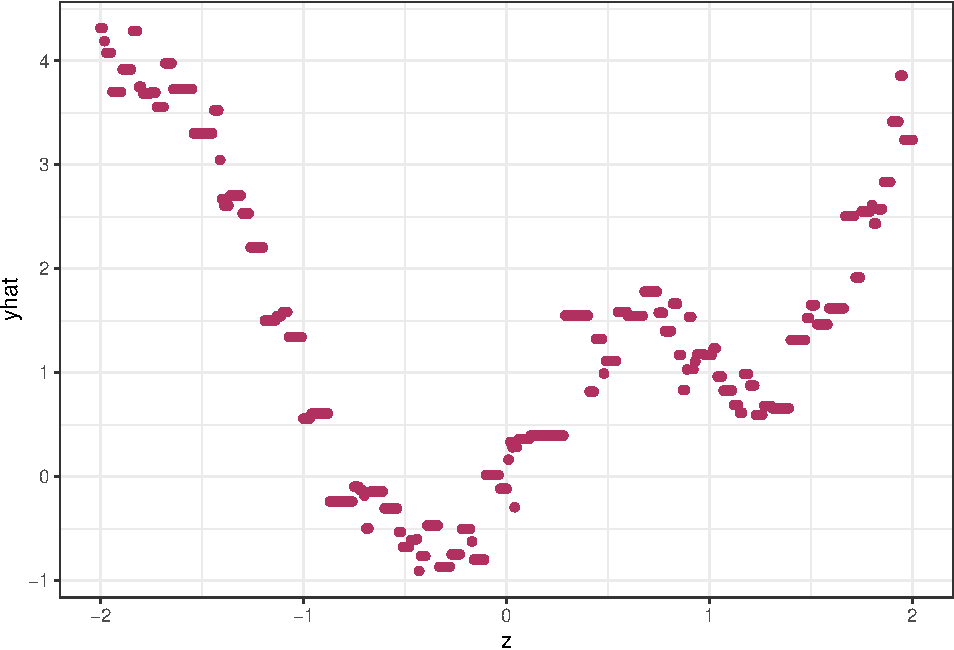
\includegraphics{hw4_files/figure-latex/unnamed-chunk-2-1.pdf}

\begin{Shaded}
\begin{Highlighting}[]
\CommentTok{# Matching Estimator (Bias-Corrected)}
\NormalTok{tau_mbc =}\StringTok{ }\KeywordTok{c}\NormalTok{()}
\NormalTok{se_tau =}\StringTok{ }\KeywordTok{c}\NormalTok{()}
\ControlFlowTok{for}\NormalTok{ (i }\ControlFlowTok{in} \DecValTok{1}\OperatorTok{:}\DecValTok{20}\NormalTok{)}
\NormalTok{\{}
\NormalTok{  model =}\StringTok{ }\KeywordTok{Match}\NormalTok{(y, z, x, }\DataTypeTok{estimand =} \StringTok{"ATE"}\NormalTok{, }\DataTypeTok{M =}\NormalTok{ i, }\DataTypeTok{BiasAdjust =}\NormalTok{ T)}
\NormalTok{  tau_mbc =}\StringTok{ }\KeywordTok{c}\NormalTok{(tau_mbc, model}\OperatorTok{\$}\NormalTok{est)}
\NormalTok{  se_tau =}\StringTok{ }\KeywordTok{c}\NormalTok{(se_tau, model}\OperatorTok{\$}\NormalTok{se)}
\NormalTok{\}}
\KeywordTok{ggplot}\NormalTok{()}\OperatorTok{+}
\StringTok{  }\KeywordTok{theme_bw}\NormalTok{() }\OperatorTok{+}
\StringTok{  }\KeywordTok{geom_point}\NormalTok{(}\KeywordTok{aes}\NormalTok{(}\DataTypeTok{x =} \DecValTok{1}\OperatorTok{:}\DecValTok{20}\NormalTok{, }\DataTypeTok{y =}\NormalTok{ tau_mbc), }\DataTypeTok{color =} \StringTok{'maroon'}\NormalTok{, }\DataTypeTok{size =} \DecValTok{2}\NormalTok{) }\OperatorTok{+}
\StringTok{  }\KeywordTok{geom_line}\NormalTok{(}\KeywordTok{aes}\NormalTok{(}\DataTypeTok{x =} \DecValTok{1}\OperatorTok{:}\DecValTok{20}\NormalTok{, }\DataTypeTok{y =}\NormalTok{ tau_mbc), }\DataTypeTok{color =} \StringTok{'maroon'}\NormalTok{, }\DataTypeTok{size =} \DecValTok{1}\NormalTok{)}
\end{Highlighting}
\end{Shaded}

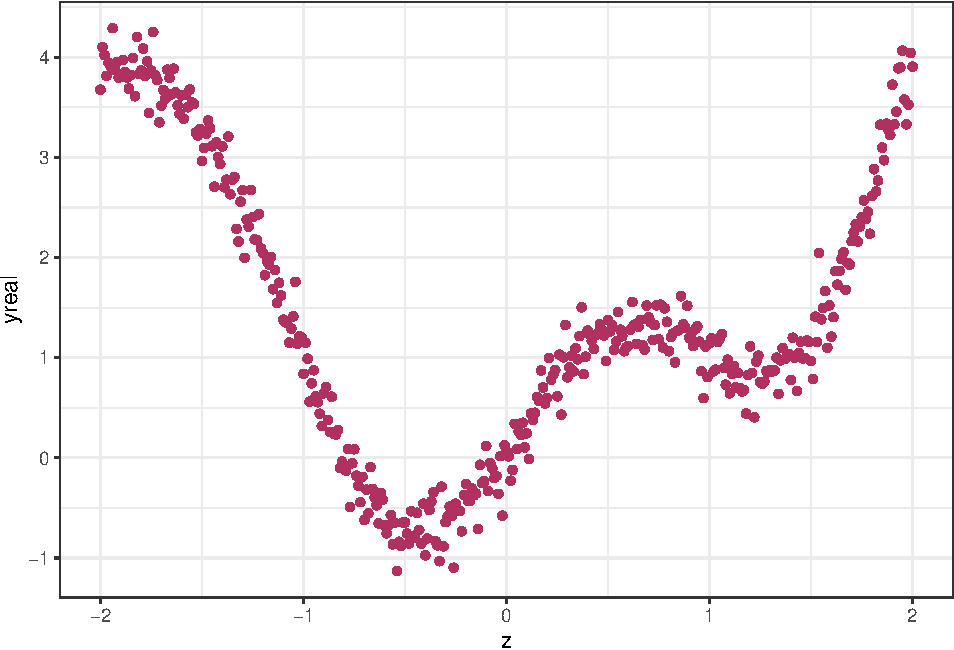
\includegraphics{hw4_files/figure-latex/unnamed-chunk-2-2.pdf}

\begin{Shaded}
\begin{Highlighting}[]
\NormalTok{karolinska =}\StringTok{ }\KeywordTok{read.table}\NormalTok{(}\StringTok{"karolinska.txt"}\NormalTok{, }\DataTypeTok{header =} \OtherTok{TRUE}\NormalTok{)}

\NormalTok{z =}\StringTok{ }\NormalTok{karolinska}\OperatorTok{\$}\NormalTok{HighVolDiagHosp}
\NormalTok{y =}\StringTok{ }\DecValTok{1} \OperatorTok{-}\StringTok{ }\NormalTok{(karolinska}\OperatorTok{\$}\NormalTok{YearsSurvivingAfterDiagnosis }\OperatorTok{==}\StringTok{ }\DecValTok{1}\NormalTok{)}
\NormalTok{x =}\StringTok{ }\KeywordTok{as.matrix}\NormalTok{(karolinska[, }\KeywordTok{c}\NormalTok{(}\DecValTok{3}\NormalTok{, }\DecValTok{4}\NormalTok{, }\DecValTok{5}\NormalTok{)])}

\NormalTok{pscore =}\StringTok{ }\KeywordTok{glm}\NormalTok{(z }\OperatorTok{~}\StringTok{ }\NormalTok{x, }\DataTypeTok{family =}\NormalTok{ binomial)}\OperatorTok{\$}\NormalTok{fitted.values}

\CommentTok{# Propensity Score Estimator}
\NormalTok{stat_SRE <-}\StringTok{ }\ControlFlowTok{function}\NormalTok{(stratum, treatment, y)\{}
  \CommentTok{# Assume in our case that the stratum in arranged and indexed.}
  \CommentTok{# If not, then re-code it to an index.}
\NormalTok{  number =}\StringTok{ }\KeywordTok{length}\NormalTok{(}\KeywordTok{unique}\NormalTok{(stratum))}
\NormalTok{  tau =}\StringTok{ }\DecValTok{0}
\NormalTok{  wil =}\StringTok{ }\DecValTok{0}
\NormalTok{  r =}\StringTok{ }\DecValTok{0}
  \CommentTok{# Calculate the three statistics as defined}
  \ControlFlowTok{for}\NormalTok{ (i }\ControlFlowTok{in} \DecValTok{1}\OperatorTok{:}\NormalTok{number)\{}
\NormalTok{    tempy =}\StringTok{ }\NormalTok{y[stratum }\OperatorTok{==}\StringTok{ }\NormalTok{i]}
\NormalTok{    tempt =}\StringTok{ }\NormalTok{treatment[stratum }\OperatorTok{==}\StringTok{ }\NormalTok{i]}
\NormalTok{    n =}\StringTok{ }\KeywordTok{length}\NormalTok{(tempy)}
\NormalTok{    pi =}\StringTok{ }\NormalTok{n}\OperatorTok{/}\KeywordTok{length}\NormalTok{(y)}
\NormalTok{    tau =}\StringTok{ }\NormalTok{tau }\OperatorTok{+}\StringTok{ }\NormalTok{pi}\OperatorTok{*}\NormalTok{(}\KeywordTok{mean}\NormalTok{(tempy[tempt }\OperatorTok{==}\StringTok{ }\DecValTok{1}\NormalTok{] }\OperatorTok{-}\StringTok{ }\KeywordTok{mean}\NormalTok{(tempy[tempt }\OperatorTok{==}\StringTok{ }\DecValTok{0}\NormalTok{])))}
\NormalTok{    tempy =}\StringTok{ }\NormalTok{tempy }\OperatorTok{-}\StringTok{ }\KeywordTok{mean}\NormalTok{(tempy)}
\NormalTok{  \}}
\NormalTok{  y <-}\StringTok{ }\KeywordTok{rank}\NormalTok{(y)}
  \ControlFlowTok{for}\NormalTok{ (i }\ControlFlowTok{in} \DecValTok{1}\OperatorTok{:}\KeywordTok{length}\NormalTok{(y))\{}
    \ControlFlowTok{if}\NormalTok{ (treatment[i] }\OperatorTok{==}\StringTok{ }\DecValTok{1}\NormalTok{)\{}
\NormalTok{      r =}\StringTok{ }\NormalTok{r }\OperatorTok{+}\StringTok{ }\NormalTok{y[i]}
\NormalTok{    \}}
\NormalTok{  \}}
  \KeywordTok{return}\NormalTok{(}\KeywordTok{c}\NormalTok{(}\DataTypeTok{taus =}\NormalTok{ tau, }\DataTypeTok{alignedRank =}\NormalTok{ r))}
\NormalTok{\}}
\CommentTok{# Here we obtain the obs. values}
\NormalTok{tau_pSRE =}\StringTok{ }\KeywordTok{c}\NormalTok{()}
\ControlFlowTok{for}\NormalTok{ (i }\ControlFlowTok{in} \DecValTok{1}\OperatorTok{:}\DecValTok{4}\NormalTok{)\{}
\NormalTok{  stratum =}\StringTok{ }\KeywordTok{floor}\NormalTok{(pscore}\OperatorTok{*}\NormalTok{i) }\OperatorTok{+}\StringTok{ }\DecValTok{1}
\NormalTok{  obsValue <-}\StringTok{ }\KeywordTok{stat_SRE}\NormalTok{(stratum, z, y)}
\NormalTok{  tau_pSRE =}\StringTok{ }\KeywordTok{c}\NormalTok{(tau_pSRE, obsValue[}\DecValTok{1}\NormalTok{])}
\NormalTok{\}}
\KeywordTok{ggplot}\NormalTok{()}\OperatorTok{+}
\StringTok{  }\KeywordTok{theme_bw}\NormalTok{() }\OperatorTok{+}
\StringTok{  }\KeywordTok{geom_point}\NormalTok{(}\KeywordTok{aes}\NormalTok{(}\DataTypeTok{x =} \DecValTok{1}\OperatorTok{:}\DecValTok{4}\NormalTok{, }\DataTypeTok{y =}\NormalTok{ tau_pSRE), }\DataTypeTok{color =} \StringTok{'maroon'}\NormalTok{, }\DataTypeTok{size =} \DecValTok{2}\NormalTok{) }\OperatorTok{+}
\StringTok{  }\KeywordTok{geom_line}\NormalTok{(}\KeywordTok{aes}\NormalTok{(}\DataTypeTok{x =} \DecValTok{1}\OperatorTok{:}\DecValTok{4}\NormalTok{, }\DataTypeTok{y =}\NormalTok{ tau_pSRE), }\DataTypeTok{color =} \StringTok{'maroon'}\NormalTok{, }\DataTypeTok{size =} \DecValTok{1}\NormalTok{)}
\end{Highlighting}
\end{Shaded}

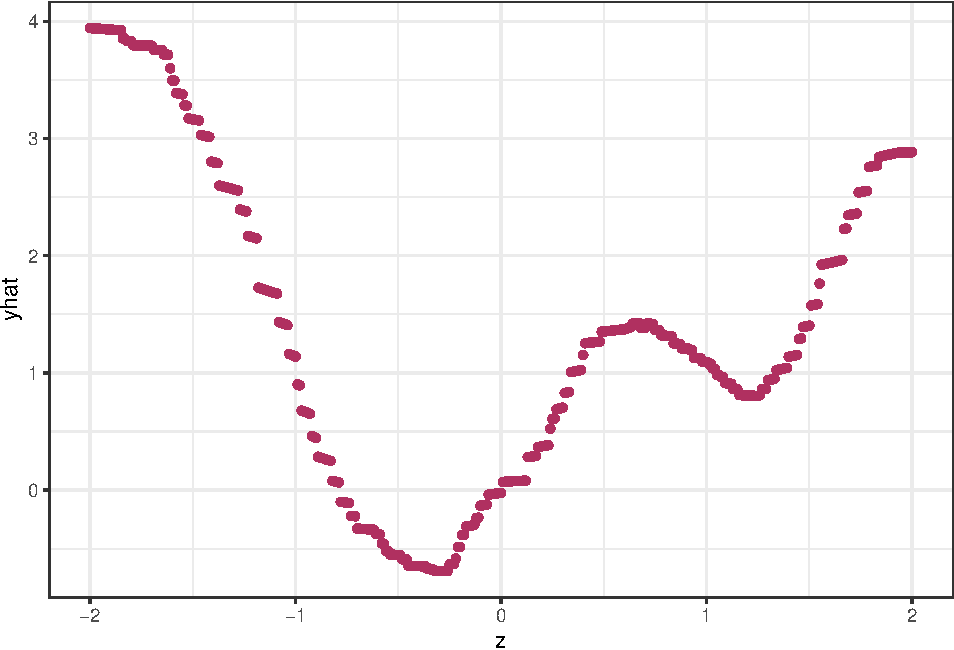
\includegraphics{hw4_files/figure-latex/unnamed-chunk-3-1.pdf}

\begin{Shaded}
\begin{Highlighting}[]
\CommentTok{# Matching Estimator (Bias-Corrected)}
\NormalTok{tau_mbc =}\StringTok{ }\KeywordTok{c}\NormalTok{()}
\NormalTok{se_tau =}\StringTok{ }\KeywordTok{c}\NormalTok{()}
\ControlFlowTok{for}\NormalTok{ (i }\ControlFlowTok{in} \DecValTok{1}\OperatorTok{:}\DecValTok{20}\NormalTok{)}
\NormalTok{\{}
\NormalTok{  model =}\StringTok{ }\KeywordTok{Match}\NormalTok{(y, z, x, }\DataTypeTok{estimand =} \StringTok{"ATE"}\NormalTok{, }\DataTypeTok{M =}\NormalTok{ i, }\DataTypeTok{BiasAdjust =}\NormalTok{ T)}
\NormalTok{  tau_mbc =}\StringTok{ }\KeywordTok{c}\NormalTok{(tau_mbc, model}\OperatorTok{\$}\NormalTok{est)}
\NormalTok{  se_tau =}\StringTok{ }\KeywordTok{c}\NormalTok{(se_tau, model}\OperatorTok{\$}\NormalTok{se)}
\NormalTok{\}}
\KeywordTok{ggplot}\NormalTok{()}\OperatorTok{+}
\StringTok{  }\KeywordTok{theme_bw}\NormalTok{() }\OperatorTok{+}
\StringTok{  }\KeywordTok{geom_point}\NormalTok{(}\KeywordTok{aes}\NormalTok{(}\DataTypeTok{x =} \DecValTok{1}\OperatorTok{:}\DecValTok{20}\NormalTok{, }\DataTypeTok{y =}\NormalTok{ tau_mbc), }\DataTypeTok{color =} \StringTok{'maroon'}\NormalTok{, }\DataTypeTok{size =} \DecValTok{2}\NormalTok{) }\OperatorTok{+}
\StringTok{  }\KeywordTok{geom_line}\NormalTok{(}\KeywordTok{aes}\NormalTok{(}\DataTypeTok{x =} \DecValTok{1}\OperatorTok{:}\DecValTok{20}\NormalTok{, }\DataTypeTok{y =}\NormalTok{ tau_mbc), }\DataTypeTok{color =} \StringTok{'maroon'}\NormalTok{, }\DataTypeTok{size =} \DecValTok{1}\NormalTok{)}
\end{Highlighting}
\end{Shaded}

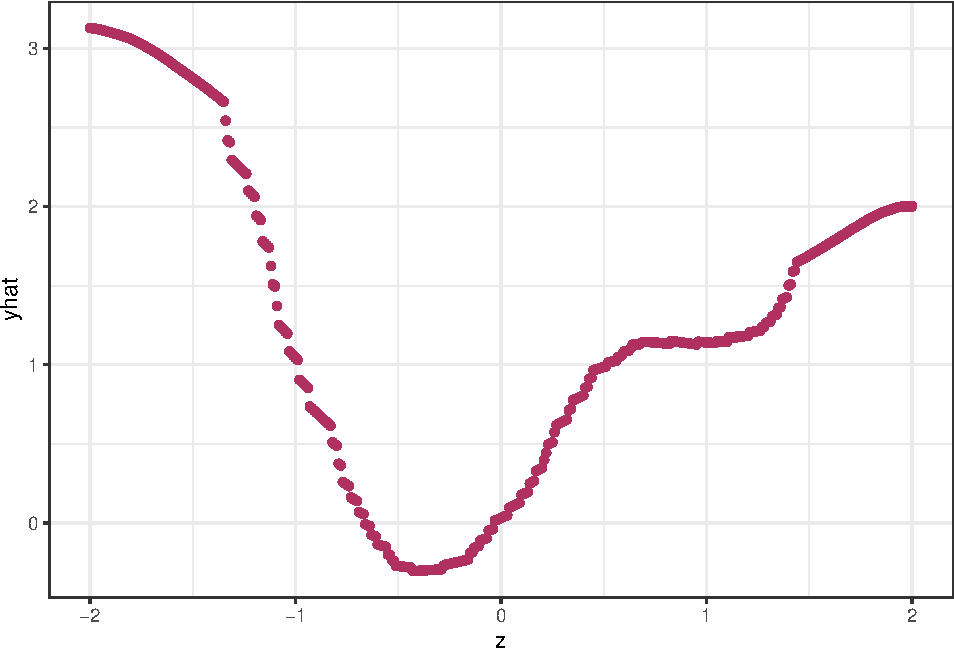
\includegraphics{hw4_files/figure-latex/unnamed-chunk-3-2.pdf}

\begin{Shaded}
\begin{Highlighting}[]
\KeywordTok{library}\NormalTok{(}\StringTok{"car"}\NormalTok{)}
\end{Highlighting}
\end{Shaded}

\begin{verbatim}
## Warning: package 'car' was built under R version 3.5.2
\end{verbatim}

\begin{verbatim}
## Loading required package: carData
\end{verbatim}

\begin{verbatim}
## 
## Attaching package: 'car'
\end{verbatim}

\begin{verbatim}
## The following object is masked from 'package:dplyr':
## 
##     recode
\end{verbatim}

\begin{verbatim}
## The following object is masked from 'package:purrr':
## 
##     some
\end{verbatim}

\begin{Shaded}
\begin{Highlighting}[]
\KeywordTok{library}\NormalTok{(}\StringTok{"Matching"}\NormalTok{)}

\NormalTok{## experimental data}
\NormalTok{lalonde =}\StringTok{ }\KeywordTok{read.csv}\NormalTok{(}\StringTok{"cps1re74.csv"}\NormalTok{, }\DataTypeTok{sep =} \StringTok{" "}\NormalTok{)}

\NormalTok{y =}\StringTok{ }\NormalTok{lalonde}\OperatorTok{\$}\NormalTok{re78}
\NormalTok{z =}\StringTok{ }\NormalTok{lalonde}\OperatorTok{\$}\NormalTok{treat}
\NormalTok{x =}\StringTok{ }\KeywordTok{as.matrix}\NormalTok{(lalonde[, }\KeywordTok{c}\NormalTok{(}\StringTok{"age"}\NormalTok{, }\StringTok{"educ"}\NormalTok{, }\StringTok{"black"}\NormalTok{,}
                          \StringTok{"hispan"}\NormalTok{, }\StringTok{"married"}\NormalTok{, }\StringTok{"nodegree"}\NormalTok{,}
                          \StringTok{"re74"}\NormalTok{, }\StringTok{"re75"}\NormalTok{)])}

\NormalTok{## analysis the randomized experiment via}
\CommentTok{# Lin's Estimator}
\NormalTok{xc =}\StringTok{ }\KeywordTok{scale}\NormalTok{(x)}
\NormalTok{linols =}\StringTok{ }\KeywordTok{lm}\NormalTok{(y }\OperatorTok{~}\StringTok{ }\NormalTok{z }\OperatorTok{+}\StringTok{ }\NormalTok{xc }\OperatorTok{+}\StringTok{ }\NormalTok{z}\OperatorTok{*}\NormalTok{xc)}
\NormalTok{tau_Lin =}\StringTok{ }\NormalTok{linols}\OperatorTok{\$}\NormalTok{coefficients[}\DecValTok{2}\NormalTok{]}
\KeywordTok{round}\NormalTok{(}\KeywordTok{summary}\NormalTok{(linols)}\OperatorTok{\$}\NormalTok{coef[}\DecValTok{2}\NormalTok{, ], }\DecValTok{4}\NormalTok{)}
\end{Highlighting}
\end{Shaded}

\begin{verbatim}
##   Estimate Std. Error    t value   Pr(>|t|) 
## -3689.8516  2457.3996    -1.5015     0.1332
\end{verbatim}

\begin{Shaded}
\begin{Highlighting}[]
\KeywordTok{sqrt}\NormalTok{(}\KeywordTok{hccm}\NormalTok{(linols)[}\DecValTok{2}\NormalTok{, }\DecValTok{2}\NormalTok{])}
\end{Highlighting}
\end{Shaded}

\begin{verbatim}
## [1] 3428.439
\end{verbatim}

\begin{Shaded}
\begin{Highlighting}[]
\CommentTok{# Regression Imputation Shall return the same results as Lin}
\NormalTok{model1 =}\StringTok{ }\KeywordTok{lm}\NormalTok{(y[z }\OperatorTok{==}\StringTok{ }\DecValTok{1}\NormalTok{]}\OperatorTok{~}\NormalTok{x[z }\OperatorTok{==}\StringTok{ }\DecValTok{1}\NormalTok{,])}
\NormalTok{model0 =}\StringTok{ }\KeywordTok{lm}\NormalTok{(y[z }\OperatorTok{==}\StringTok{ }\DecValTok{0}\NormalTok{]}\OperatorTok{~}\NormalTok{x[z }\OperatorTok{==}\StringTok{ }\DecValTok{0}\NormalTok{,])}
\NormalTok{tau_reg =}\StringTok{ }\KeywordTok{mean}\NormalTok{(}\KeywordTok{cbind}\NormalTok{(}\DecValTok{1}\NormalTok{, x) }\OperatorTok{\%*\%}\StringTok{ }\NormalTok{model1}\OperatorTok{\$}\NormalTok{coefficients }\OperatorTok{-}\StringTok{ }\KeywordTok{cbind}\NormalTok{(}\DecValTok{1}\NormalTok{, x) }\OperatorTok{\%*\%}\StringTok{ }\NormalTok{model0}\OperatorTok{\$}\NormalTok{coefficients)}
\NormalTok{tau_Lin }\OperatorTok{-}\StringTok{ }\NormalTok{tau_reg}
\end{Highlighting}
\end{Shaded}

\begin{verbatim}
##            z 
## 3.187779e-09
\end{verbatim}

\begin{Shaded}
\begin{Highlighting}[]
\CommentTok{# Propensity score stratification}
\NormalTok{pscore =}\StringTok{ }\KeywordTok{glm}\NormalTok{(z }\OperatorTok{~}\StringTok{ }\NormalTok{x, }\DataTypeTok{family =}\NormalTok{ binomial)}\OperatorTok{\$}\NormalTok{fitted.values}
\NormalTok{tau_pSRE =}\StringTok{ }\KeywordTok{c}\NormalTok{()}
\ControlFlowTok{for}\NormalTok{ (i }\ControlFlowTok{in} \DecValTok{2}\OperatorTok{:}\DecValTok{5}\NormalTok{)\{}
\NormalTok{  stratum =}\StringTok{ }\KeywordTok{floor}\NormalTok{(pscore}\OperatorTok{*}\NormalTok{i) }\OperatorTok{+}\StringTok{ }\DecValTok{1}
\NormalTok{  obsValue <-}\StringTok{ }\KeywordTok{stat_SRE}\NormalTok{(stratum, z, y)}
\NormalTok{  tau_pSRE =}\StringTok{ }\KeywordTok{c}\NormalTok{(tau_pSRE, obsValue[}\DecValTok{1}\NormalTok{])}
\NormalTok{\}}
\NormalTok{tau_pSRE}
\end{Highlighting}
\end{Shaded}

\begin{verbatim}
##      taus      taus      taus      taus 
## -8506.495 -7804.194 -7706.861 -7625.539
\end{verbatim}

\begin{Shaded}
\begin{Highlighting}[]
\CommentTok{# IPW estimator}
\CommentTok{# With no truncation}
\NormalTok{truncpscore =}\StringTok{ }\KeywordTok{c}\NormalTok{(}\DecValTok{0}\NormalTok{,}\DecValTok{1}\NormalTok{)}
\NormalTok{pscore =}\StringTok{ }\KeywordTok{glm}\NormalTok{(z }\OperatorTok{~}\StringTok{ }\NormalTok{x, }\DataTypeTok{family =}\NormalTok{ binomial)}\OperatorTok{\$}\NormalTok{fitted.values}
\NormalTok{pscore =}\StringTok{ }\KeywordTok{pmax}\NormalTok{(truncpscore[}\DecValTok{1}\NormalTok{], }\KeywordTok{pmin}\NormalTok{(truncpscore[}\DecValTok{2}\NormalTok{], pscore))}
\NormalTok{ipw_}\DecValTok{1}\NormalTok{ =}\StringTok{ }\KeywordTok{mean}\NormalTok{(z}\OperatorTok{*}\NormalTok{y}\OperatorTok{/}\NormalTok{pscore }\OperatorTok{-}\StringTok{ }\NormalTok{(}\DecValTok{1} \OperatorTok{-}\StringTok{ }\NormalTok{z)}\OperatorTok{*}\NormalTok{y}\OperatorTok{/}\NormalTok{(}\DecValTok{1} \OperatorTok{-}\StringTok{ }\NormalTok{pscore))}
\NormalTok{ipw_hajek_}\DecValTok{1}\NormalTok{ =}\StringTok{ }\KeywordTok{mean}\NormalTok{(z}\OperatorTok{*}\NormalTok{y}\OperatorTok{/}\NormalTok{pscore)}\OperatorTok{/}\KeywordTok{mean}\NormalTok{(z}\OperatorTok{/}\NormalTok{pscore) }\OperatorTok{-}\StringTok{ }\KeywordTok{mean}\NormalTok{((}\DecValTok{1} \OperatorTok{-}\StringTok{ }\NormalTok{z)}\OperatorTok{*}\NormalTok{y}\OperatorTok{/}\NormalTok{(}\DecValTok{1} \OperatorTok{-}\StringTok{ }\NormalTok{pscore))}\OperatorTok{/}\KeywordTok{mean}\NormalTok{((}\DecValTok{1} \OperatorTok{-}\StringTok{ }\NormalTok{z)}\OperatorTok{/}\NormalTok{(}\DecValTok{1} \OperatorTok{-}\StringTok{ }\NormalTok{pscore))}

\CommentTok{# With certain truncation}
\NormalTok{truncpscore =}\StringTok{ }\KeywordTok{c}\NormalTok{(}\FloatTok{0.1}\NormalTok{,}\FloatTok{0.9}\NormalTok{)}
\NormalTok{pscore =}\StringTok{ }\KeywordTok{glm}\NormalTok{(z }\OperatorTok{~}\StringTok{ }\NormalTok{x, }\DataTypeTok{family =}\NormalTok{ binomial)}\OperatorTok{\$}\NormalTok{fitted.values}
\NormalTok{pscore =}\StringTok{ }\KeywordTok{pmax}\NormalTok{(truncpscore[}\DecValTok{1}\NormalTok{], }\KeywordTok{pmin}\NormalTok{(truncpscore[}\DecValTok{2}\NormalTok{], pscore))}
\NormalTok{ipw_}\DecValTok{2}\NormalTok{ =}\StringTok{ }\KeywordTok{mean}\NormalTok{(z}\OperatorTok{*}\NormalTok{y}\OperatorTok{/}\NormalTok{pscore }\OperatorTok{-}\StringTok{ }\NormalTok{(}\DecValTok{1} \OperatorTok{-}\StringTok{ }\NormalTok{z)}\OperatorTok{*}\NormalTok{y}\OperatorTok{/}\NormalTok{(}\DecValTok{1} \OperatorTok{-}\StringTok{ }\NormalTok{pscore))}
\NormalTok{ipw_hajek_}\DecValTok{2}\NormalTok{ =}\StringTok{ }\KeywordTok{mean}\NormalTok{(z}\OperatorTok{*}\NormalTok{y}\OperatorTok{/}\NormalTok{pscore)}\OperatorTok{/}\KeywordTok{mean}\NormalTok{(z}\OperatorTok{/}\NormalTok{pscore) }\OperatorTok{-}\StringTok{ }\KeywordTok{mean}\NormalTok{((}\DecValTok{1} \OperatorTok{-}\StringTok{ }\NormalTok{z)}\OperatorTok{*}\NormalTok{y}\OperatorTok{/}\NormalTok{(}\DecValTok{1} \OperatorTok{-}\StringTok{ }\NormalTok{pscore))}\OperatorTok{/}\KeywordTok{mean}\NormalTok{((}\DecValTok{1} \OperatorTok{-}\StringTok{ }\NormalTok{z)}\OperatorTok{/}\NormalTok{(}\DecValTok{1} \OperatorTok{-}\StringTok{ }\NormalTok{pscore))}

\CommentTok{# Doubly Robust Estimator}
\NormalTok{outcome1 =}\StringTok{ }\KeywordTok{glm}\NormalTok{(y }\OperatorTok{~}\StringTok{ }\NormalTok{x, }\DataTypeTok{weights =}\NormalTok{ z, }\DataTypeTok{family =}\NormalTok{ gaussian)}\OperatorTok{\$}\NormalTok{fitted.values}
\NormalTok{outcome0 =}\StringTok{ }\KeywordTok{glm}\NormalTok{(y }\OperatorTok{~}\StringTok{ }\NormalTok{x, }\DataTypeTok{weights =}\NormalTok{ (}\DecValTok{1} \OperatorTok{-}\StringTok{ }\NormalTok{z), }\DataTypeTok{family =}\NormalTok{ gaussian)}\OperatorTok{\$}\NormalTok{fitted.values}
\NormalTok{res1 =}\StringTok{ }\NormalTok{y }\OperatorTok{-}\StringTok{ }\NormalTok{outcome1}
\NormalTok{res0 =}\StringTok{ }\NormalTok{y }\OperatorTok{-}\StringTok{ }\NormalTok{outcome0}
\NormalTok{tau_dr =}\StringTok{ }\KeywordTok{mean}\NormalTok{(outcome1 }\OperatorTok{-}\StringTok{ }\NormalTok{outcome0) }\OperatorTok{+}\StringTok{ }\KeywordTok{mean}\NormalTok{(z}\OperatorTok{*}\NormalTok{res1}\OperatorTok{/}\NormalTok{pscore }\OperatorTok{-}\StringTok{ }\NormalTok{(}\DecValTok{1} \OperatorTok{-}\StringTok{ }\NormalTok{z)}\OperatorTok{*}\NormalTok{res0}\OperatorTok{/}\NormalTok{(}\DecValTok{1} \OperatorTok{-}\StringTok{ }\NormalTok{pscore))}

\KeywordTok{print}\NormalTok{(}\KeywordTok{paste}\NormalTok{(}\StringTok{"Lin's estimator is "}\NormalTok{, tau_Lin, }\DataTypeTok{sep =} \StringTok{""}\NormalTok{))}
\end{Highlighting}
\end{Shaded}

\begin{verbatim}
## [1] "Lin's estimator is -3689.8515880728"
\end{verbatim}

\begin{Shaded}
\begin{Highlighting}[]
\KeywordTok{print}\NormalTok{(}\KeywordTok{paste}\NormalTok{(}\StringTok{"Regression Imputation gives us an estimate same as Lin's "}\NormalTok{, tau_reg, }\DataTypeTok{sep =} \StringTok{""}\NormalTok{))}
\end{Highlighting}
\end{Shaded}

\begin{verbatim}
## [1] "Regression Imputation gives us an estimate same as Lin's -3689.85158807599"
\end{verbatim}

\begin{Shaded}
\begin{Highlighting}[]
\KeywordTok{print}\NormalTok{(}\KeywordTok{paste}\NormalTok{(}\StringTok{"pscore stratification's estimator is "}\NormalTok{, tau_pSRE, }\DataTypeTok{sep =} \StringTok{""}\NormalTok{))}
\end{Highlighting}
\end{Shaded}

\begin{verbatim}
## [1] "pscore stratification's estimator is -8506.49536105039"
## [2] "pscore stratification's estimator is -7804.1941784074" 
## [3] "pscore stratification's estimator is -7706.8611458836" 
## [4] "pscore stratification's estimator is -7625.53852433987"
\end{verbatim}

\begin{Shaded}
\begin{Highlighting}[]
\KeywordTok{print}\NormalTok{(}\KeywordTok{paste}\NormalTok{(}\StringTok{"IPW estimator (hovic-thompson) without truncation is "}\NormalTok{,ipw_}\DecValTok{1}\NormalTok{, }\StringTok{" and the hajek estimator is "}\NormalTok{,ipw_hajek_}\DecValTok{1}\NormalTok{ ,}\DataTypeTok{sep =} \StringTok{""}\NormalTok{))}
\end{Highlighting}
\end{Shaded}

\begin{verbatim}
## [1] "IPW estimator (hovic-thompson) without truncation is -10452.7456142986 and the hajek estimator is -6464.79903460242"
\end{verbatim}

\begin{Shaded}
\begin{Highlighting}[]
\KeywordTok{print}\NormalTok{(}\KeywordTok{paste}\NormalTok{(}\StringTok{"IPW estimator (hovic-thompson) with truncation is "}\NormalTok{,ipw_}\DecValTok{2}\NormalTok{, }\StringTok{" and the hajek estimator is "}\NormalTok{,ipw_hajek_}\DecValTok{2}\NormalTok{ ,}\DataTypeTok{sep =} \StringTok{""}\NormalTok{))}
\end{Highlighting}
\end{Shaded}

\begin{verbatim}
## [1] "IPW estimator (hovic-thompson) with truncation is -15955.5388374637 and the hajek estimator is -7870.10636452558"
\end{verbatim}

\begin{Shaded}
\begin{Highlighting}[]
\KeywordTok{print}\NormalTok{(}\KeywordTok{paste}\NormalTok{(}\StringTok{"The doubly robust estimator is "}\NormalTok{, tau_dr))}
\end{Highlighting}
\end{Shaded}

\begin{verbatim}
## [1] "The doubly robust estimator is  -3688.65001081252"
\end{verbatim}

\begin{Shaded}
\begin{Highlighting}[]
\CommentTok{# Propensity score stratification}
\NormalTok{pscore =}\StringTok{ }\KeywordTok{glm}\NormalTok{(z }\OperatorTok{~}\StringTok{ }\NormalTok{x, }\DataTypeTok{family =} \KeywordTok{binomial}\NormalTok{(}\DataTypeTok{link =} \StringTok{"probit"}\NormalTok{))}\OperatorTok{\$}\NormalTok{fitted.values}
\NormalTok{tau_pSRE =}\StringTok{ }\KeywordTok{c}\NormalTok{()}
\ControlFlowTok{for}\NormalTok{ (i }\ControlFlowTok{in} \DecValTok{2}\OperatorTok{:}\DecValTok{5}\NormalTok{)\{}
\NormalTok{  stratum =}\StringTok{ }\KeywordTok{floor}\NormalTok{(pscore}\OperatorTok{*}\NormalTok{i) }\OperatorTok{+}\StringTok{ }\DecValTok{1}
\NormalTok{  obsValue <-}\StringTok{ }\KeywordTok{stat_SRE}\NormalTok{(stratum, z, y)}
\NormalTok{  tau_pSRE =}\StringTok{ }\KeywordTok{c}\NormalTok{(tau_pSRE, obsValue[}\DecValTok{1}\NormalTok{])}
\NormalTok{\}}

\CommentTok{# IPW estimator}
\CommentTok{# With no truncation}
\NormalTok{truncpscore =}\StringTok{ }\KeywordTok{c}\NormalTok{(}\DecValTok{0}\NormalTok{,}\DecValTok{1}\NormalTok{)}
\NormalTok{pscore =}\StringTok{ }\KeywordTok{glm}\NormalTok{(z }\OperatorTok{~}\StringTok{ }\NormalTok{x, }\DataTypeTok{family =} \KeywordTok{binomial}\NormalTok{(}\DataTypeTok{link =} \StringTok{"probit"}\NormalTok{))}\OperatorTok{\$}\NormalTok{fitted.values}
\NormalTok{pscore =}\StringTok{ }\KeywordTok{pmax}\NormalTok{(truncpscore[}\DecValTok{1}\NormalTok{], }\KeywordTok{pmin}\NormalTok{(truncpscore[}\DecValTok{2}\NormalTok{], pscore))}
\NormalTok{ipw_}\DecValTok{1}\NormalTok{ =}\StringTok{ }\KeywordTok{mean}\NormalTok{(z}\OperatorTok{*}\NormalTok{y}\OperatorTok{/}\NormalTok{pscore }\OperatorTok{-}\StringTok{ }\NormalTok{(}\DecValTok{1} \OperatorTok{-}\StringTok{ }\NormalTok{z)}\OperatorTok{*}\NormalTok{y}\OperatorTok{/}\NormalTok{(}\DecValTok{1} \OperatorTok{-}\StringTok{ }\NormalTok{pscore))}
\NormalTok{ipw_hajek_}\DecValTok{1}\NormalTok{ =}\StringTok{ }\KeywordTok{mean}\NormalTok{(z}\OperatorTok{*}\NormalTok{y}\OperatorTok{/}\NormalTok{pscore)}\OperatorTok{/}\KeywordTok{mean}\NormalTok{(z}\OperatorTok{/}\NormalTok{pscore) }\OperatorTok{-}\StringTok{ }\KeywordTok{mean}\NormalTok{((}\DecValTok{1} \OperatorTok{-}\StringTok{ }\NormalTok{z)}\OperatorTok{*}\NormalTok{y}\OperatorTok{/}\NormalTok{(}\DecValTok{1} \OperatorTok{-}\StringTok{ }\NormalTok{pscore))}\OperatorTok{/}\KeywordTok{mean}\NormalTok{((}\DecValTok{1} \OperatorTok{-}\StringTok{ }\NormalTok{z)}\OperatorTok{/}\NormalTok{(}\DecValTok{1} \OperatorTok{-}\StringTok{ }\NormalTok{pscore))}

\CommentTok{# With certain truncation}
\NormalTok{truncpscore =}\StringTok{ }\KeywordTok{c}\NormalTok{(}\FloatTok{0.1}\NormalTok{,}\FloatTok{0.9}\NormalTok{)}
\NormalTok{pscore =}\StringTok{ }\KeywordTok{glm}\NormalTok{(z }\OperatorTok{~}\StringTok{ }\NormalTok{x, }\DataTypeTok{family =} \KeywordTok{binomial}\NormalTok{(}\DataTypeTok{link =} \StringTok{"probit"}\NormalTok{))}\OperatorTok{\$}\NormalTok{fitted.values}
\NormalTok{pscore =}\StringTok{ }\KeywordTok{pmax}\NormalTok{(truncpscore[}\DecValTok{1}\NormalTok{], }\KeywordTok{pmin}\NormalTok{(truncpscore[}\DecValTok{2}\NormalTok{], pscore))}
\NormalTok{ipw_}\DecValTok{2}\NormalTok{ =}\StringTok{ }\KeywordTok{mean}\NormalTok{(z}\OperatorTok{*}\NormalTok{y}\OperatorTok{/}\NormalTok{pscore }\OperatorTok{-}\StringTok{ }\NormalTok{(}\DecValTok{1} \OperatorTok{-}\StringTok{ }\NormalTok{z)}\OperatorTok{*}\NormalTok{y}\OperatorTok{/}\NormalTok{(}\DecValTok{1} \OperatorTok{-}\StringTok{ }\NormalTok{pscore))}
\NormalTok{ipw_hajek_}\DecValTok{2}\NormalTok{ =}\StringTok{ }\KeywordTok{mean}\NormalTok{(z}\OperatorTok{*}\NormalTok{y}\OperatorTok{/}\NormalTok{pscore)}\OperatorTok{/}\KeywordTok{mean}\NormalTok{(z}\OperatorTok{/}\NormalTok{pscore) }\OperatorTok{-}\StringTok{ }\KeywordTok{mean}\NormalTok{((}\DecValTok{1} \OperatorTok{-}\StringTok{ }\NormalTok{z)}\OperatorTok{*}\NormalTok{y}\OperatorTok{/}\NormalTok{(}\DecValTok{1} \OperatorTok{-}\StringTok{ }\NormalTok{pscore))}\OperatorTok{/}\KeywordTok{mean}\NormalTok{((}\DecValTok{1} \OperatorTok{-}\StringTok{ }\NormalTok{z)}\OperatorTok{/}\NormalTok{(}\DecValTok{1} \OperatorTok{-}\StringTok{ }\NormalTok{pscore))}

\CommentTok{# Doubly Robust Estimator}
\NormalTok{outcome1 =}\StringTok{ }\KeywordTok{glm}\NormalTok{(y }\OperatorTok{~}\StringTok{ }\NormalTok{x, }\DataTypeTok{weights =}\NormalTok{ z, }\DataTypeTok{family =}\NormalTok{ gaussian)}\OperatorTok{\$}\NormalTok{fitted.values}
\NormalTok{outcome0 =}\StringTok{ }\KeywordTok{glm}\NormalTok{(y }\OperatorTok{~}\StringTok{ }\NormalTok{x, }\DataTypeTok{weights =}\NormalTok{ (}\DecValTok{1} \OperatorTok{-}\StringTok{ }\NormalTok{z), }\DataTypeTok{family =}\NormalTok{ gaussian)}\OperatorTok{\$}\NormalTok{fitted.values}
\NormalTok{res1 =}\StringTok{ }\NormalTok{y }\OperatorTok{-}\StringTok{ }\NormalTok{outcome1}
\NormalTok{res0 =}\StringTok{ }\NormalTok{y }\OperatorTok{-}\StringTok{ }\NormalTok{outcome0}
\NormalTok{tau_dr =}\StringTok{ }\KeywordTok{mean}\NormalTok{(outcome1 }\OperatorTok{-}\StringTok{ }\NormalTok{outcome0) }\OperatorTok{+}\StringTok{ }\KeywordTok{mean}\NormalTok{(z}\OperatorTok{*}\NormalTok{res1}\OperatorTok{/}\NormalTok{pscore }\OperatorTok{-}\StringTok{ }\NormalTok{(}\DecValTok{1} \OperatorTok{-}\StringTok{ }\NormalTok{z)}\OperatorTok{*}\NormalTok{res0}\OperatorTok{/}\NormalTok{(}\DecValTok{1} \OperatorTok{-}\StringTok{ }\NormalTok{pscore))}

\KeywordTok{print}\NormalTok{(}\StringTok{"If we fit e(x) by probit model,"}\NormalTok{)}
\end{Highlighting}
\end{Shaded}

\begin{verbatim}
## [1] "If we fit e(x) by probit model,"
\end{verbatim}

\begin{Shaded}
\begin{Highlighting}[]
\KeywordTok{print}\NormalTok{(}\KeywordTok{paste}\NormalTok{(}\StringTok{"Lin's estimator is "}\NormalTok{, tau_Lin, }\DataTypeTok{sep =} \StringTok{""}\NormalTok{))}
\end{Highlighting}
\end{Shaded}

\begin{verbatim}
## [1] "Lin's estimator is -3689.8515880728"
\end{verbatim}

\begin{Shaded}
\begin{Highlighting}[]
\KeywordTok{print}\NormalTok{(}\KeywordTok{paste}\NormalTok{(}\StringTok{"Regression Imputation gives us an estimate same as Lin's "}\NormalTok{, tau_reg, }\DataTypeTok{sep =} \StringTok{""}\NormalTok{))}
\end{Highlighting}
\end{Shaded}

\begin{verbatim}
## [1] "Regression Imputation gives us an estimate same as Lin's -3689.85158807599"
\end{verbatim}

\begin{Shaded}
\begin{Highlighting}[]
\KeywordTok{print}\NormalTok{(}\KeywordTok{paste}\NormalTok{(}\StringTok{"pscore stratification's estimator is "}\NormalTok{, tau_pSRE, }\DataTypeTok{sep =} \StringTok{""}\NormalTok{))}
\end{Highlighting}
\end{Shaded}

\begin{verbatim}
## [1] "pscore stratification's estimator is -8506.49536105039"
## [2] "pscore stratification's estimator is -7826.07775869297"
## [3] "pscore stratification's estimator is -7199.12284967037"
## [4] "pscore stratification's estimator is -7185.93488163915"
\end{verbatim}

\begin{Shaded}
\begin{Highlighting}[]
\KeywordTok{print}\NormalTok{(}\KeywordTok{paste}\NormalTok{(}\StringTok{"IPW estimator (hovic-thompson) without truncation is "}\NormalTok{,ipw_}\DecValTok{1}\NormalTok{, }\StringTok{" and the hajek estimator is "}\NormalTok{,ipw_hajek_}\DecValTok{1}\NormalTok{ ,}\DataTypeTok{sep =} \StringTok{""}\NormalTok{))}
\end{Highlighting}
\end{Shaded}

\begin{verbatim}
## [1] "IPW estimator (hovic-thompson) without truncation is -8738.13952518101 and the hajek estimator is -6452.09781690384"
\end{verbatim}

\begin{Shaded}
\begin{Highlighting}[]
\KeywordTok{print}\NormalTok{(}\KeywordTok{paste}\NormalTok{(}\StringTok{"IPW estimator (hovic-thompson) with truncation is "}\NormalTok{,ipw_}\DecValTok{2}\NormalTok{, }\StringTok{" and the hajek estimator is "}\NormalTok{,ipw_hajek_}\DecValTok{2}\NormalTok{ ,}\DataTypeTok{sep =} \StringTok{""}\NormalTok{))}
\end{Highlighting}
\end{Shaded}

\begin{verbatim}
## [1] "IPW estimator (hovic-thompson) with truncation is -15953.1987455341 and the hajek estimator is -7869.30235400649"
\end{verbatim}

\begin{Shaded}
\begin{Highlighting}[]
\KeywordTok{print}\NormalTok{(}\KeywordTok{paste}\NormalTok{(}\StringTok{"The doubly robust estimator is "}\NormalTok{, tau_dr))}
\end{Highlighting}
\end{Shaded}

\begin{verbatim}
## [1] "The doubly robust estimator is  -3686.27091355767"
\end{verbatim}

\begin{Shaded}
\begin{Highlighting}[]
\KeywordTok{print}\NormalTok{(}\StringTok{"The doubly robust estimator is the one closest to the golden rule estimation."}\NormalTok{)}
\end{Highlighting}
\end{Shaded}

\begin{verbatim}
## [1] "The doubly robust estimator is the one closest to the golden rule estimation."
\end{verbatim}

\begin{Shaded}
\begin{Highlighting}[]
\KeywordTok{library}\NormalTok{(MatchIt)}
\end{Highlighting}
\end{Shaded}

\begin{verbatim}
## 
## Attaching package: 'MatchIt'
\end{verbatim}

\begin{verbatim}
## The following object is masked _by_ '.GlobalEnv':
## 
##     lalonde
\end{verbatim}

\begin{Shaded}
\begin{Highlighting}[]
\NormalTok{data <-}\StringTok{ }\KeywordTok{read.csv}\NormalTok{(}\StringTok{"FDA-Carpenter.csv"}\NormalTok{)}
\CommentTok{# We perform similar data treatment }
\CommentTok{# The democrat is the senate is the treatment indicator, acttime is Y, and others are covariate.}

\NormalTok{## rescaling}
\NormalTok{data}\OperatorTok{\$}\NormalTok{hospdisc <-}\StringTok{ }\NormalTok{data}\OperatorTok{\$}\NormalTok{hospdisc}\OperatorTok{/}\DecValTok{100000}
\NormalTok{data}\OperatorTok{\$}\NormalTok{natreg <-}\StringTok{ }\NormalTok{data}\OperatorTok{\$}\NormalTok{natreg}\OperatorTok{/}\DecValTok{100}
\NormalTok{data}\OperatorTok{\$}\NormalTok{stafcder <-}\StringTok{ }\NormalTok{data}\OperatorTok{\$}\NormalTok{stafcder}\OperatorTok{/}\DecValTok{100}
\NormalTok{data}\OperatorTok{\$}\NormalTok{prevgenx <-}\StringTok{ }\NormalTok{data}\OperatorTok{\$}\NormalTok{prevgenx}\OperatorTok{/}\DecValTok{100}
\NormalTok{data}\OperatorTok{\$}\NormalTok{hhosleng <-}\StringTok{ }\NormalTok{data}\OperatorTok{\$}\NormalTok{hhosleng}\OperatorTok{/}\DecValTok{10}
\NormalTok{data}\OperatorTok{\$}\NormalTok{condavg3 <-}\StringTok{ }\NormalTok{data}\OperatorTok{\$}\NormalTok{condavg3}\OperatorTok{/}\DecValTok{10}
\NormalTok{data}\OperatorTok{\$}\NormalTok{orderent <-}\StringTok{ }\NormalTok{data}\OperatorTok{\$}\NormalTok{orderent}\OperatorTok{/}\DecValTok{10}
\NormalTok{data}\OperatorTok{\$}\NormalTok{vandavg3 <-}\StringTok{ }\NormalTok{data}\OperatorTok{\$}\NormalTok{vandavg3}\OperatorTok{/}\DecValTok{10}
\NormalTok{data}\OperatorTok{\$}\NormalTok{wpnoavg3 <-}\StringTok{ }\NormalTok{data}\OperatorTok{\$}\NormalTok{wpnoavg3}\OperatorTok{/}\DecValTok{100}

\NormalTok{z <-}\StringTok{ }\NormalTok{data}\OperatorTok{\$}\NormalTok{demsnmaj}
\NormalTok{y <-}\StringTok{ }\NormalTok{data}\OperatorTok{\$}\NormalTok{acttime}
\NormalTok{x <-}\StringTok{ }\KeywordTok{as.matrix}\NormalTok{(data }\OperatorTok{\%>\%}
\StringTok{  }\NormalTok{dplyr}\OperatorTok{::}\KeywordTok{select}\NormalTok{(}\OperatorTok{-}\NormalTok{demsnmaj, }\OperatorTok{-}\NormalTok{acttime))}
\NormalTok{## analysis the randomized experiment via}
\CommentTok{# Lin's Estimator}
\NormalTok{xc =}\StringTok{ }\KeywordTok{scale}\NormalTok{(x)}
\NormalTok{linols =}\StringTok{ }\KeywordTok{lm}\NormalTok{(y }\OperatorTok{~}\StringTok{ }\NormalTok{z }\OperatorTok{+}\StringTok{ }\NormalTok{xc }\OperatorTok{+}\StringTok{ }\NormalTok{z}\OperatorTok{*}\NormalTok{xc)}
\NormalTok{tau_Lin =}\StringTok{ }\NormalTok{linols}\OperatorTok{\$}\NormalTok{coefficients[}\DecValTok{2}\NormalTok{]}
\KeywordTok{round}\NormalTok{(}\KeywordTok{summary}\NormalTok{(linols)}\OperatorTok{\$}\NormalTok{coef[}\DecValTok{2}\NormalTok{, ], }\DecValTok{4}\NormalTok{)}
\end{Highlighting}
\end{Shaded}

\begin{verbatim}
##   Estimate Std. Error    t value   Pr(>|t|) 
##   -13.8625     4.4678    -3.1027     0.0021
\end{verbatim}

\begin{Shaded}
\begin{Highlighting}[]
\KeywordTok{sqrt}\NormalTok{(}\KeywordTok{hccm}\NormalTok{(linols)[}\DecValTok{2}\NormalTok{, }\DecValTok{2}\NormalTok{])}
\end{Highlighting}
\end{Shaded}

\begin{verbatim}
## [1] 4.389857
\end{verbatim}

\begin{Shaded}
\begin{Highlighting}[]
\CommentTok{# Regression Imputation Shall return the same results as Lin}
\NormalTok{model1 =}\StringTok{ }\KeywordTok{lm}\NormalTok{(y[z }\OperatorTok{==}\StringTok{ }\DecValTok{1}\NormalTok{]}\OperatorTok{~}\NormalTok{x[z }\OperatorTok{==}\StringTok{ }\DecValTok{1}\NormalTok{,])}
\NormalTok{model0 =}\StringTok{ }\KeywordTok{lm}\NormalTok{(y[z }\OperatorTok{==}\StringTok{ }\DecValTok{0}\NormalTok{]}\OperatorTok{~}\NormalTok{x[z }\OperatorTok{==}\StringTok{ }\DecValTok{0}\NormalTok{,])}
\NormalTok{tau_reg =}\StringTok{ }\KeywordTok{mean}\NormalTok{(}\KeywordTok{cbind}\NormalTok{(}\DecValTok{1}\NormalTok{, x) }\OperatorTok{\%*\%}\StringTok{ }\NormalTok{model1}\OperatorTok{\$}\NormalTok{coefficients }\OperatorTok{-}\StringTok{ }\KeywordTok{cbind}\NormalTok{(}\DecValTok{1}\NormalTok{, x) }\OperatorTok{\%*\%}\StringTok{ }\NormalTok{model0}\OperatorTok{\$}\NormalTok{coefficients)}

\CommentTok{# Propensity score stratification}
\NormalTok{pscore =}\StringTok{ }\KeywordTok{glm}\NormalTok{(z }\OperatorTok{~}\StringTok{ }\NormalTok{x, }\DataTypeTok{family =}\NormalTok{ binomial)}\OperatorTok{\$}\NormalTok{fitted.values}
\NormalTok{tau_pSRE =}\StringTok{ }\KeywordTok{c}\NormalTok{()}
\ControlFlowTok{for}\NormalTok{ (i }\ControlFlowTok{in} \DecValTok{2}\OperatorTok{:}\DecValTok{5}\NormalTok{)\{}
\NormalTok{  stratum =}\StringTok{ }\KeywordTok{floor}\NormalTok{(pscore}\OperatorTok{*}\NormalTok{i) }\OperatorTok{+}\StringTok{ }\DecValTok{1}
\NormalTok{  obsValue <-}\StringTok{ }\KeywordTok{stat_SRE}\NormalTok{(stratum, z, y)}
\NormalTok{  tau_pSRE =}\StringTok{ }\KeywordTok{c}\NormalTok{(tau_pSRE, obsValue[}\DecValTok{1}\NormalTok{])}
\NormalTok{\}}
\NormalTok{tau_pSRE}
\end{Highlighting}
\end{Shaded}

\begin{verbatim}
##      taus      taus      taus      taus 
## -11.78213 -13.49131 -14.69429 -16.93254
\end{verbatim}

\begin{Shaded}
\begin{Highlighting}[]
\CommentTok{# IPW estimator}
\CommentTok{# With no truncation}
\NormalTok{truncpscore =}\StringTok{ }\KeywordTok{c}\NormalTok{(}\DecValTok{0}\NormalTok{,}\DecValTok{1}\NormalTok{)}
\NormalTok{pscore =}\StringTok{ }\KeywordTok{glm}\NormalTok{(z }\OperatorTok{~}\StringTok{ }\NormalTok{x, }\DataTypeTok{family =}\NormalTok{ binomial)}\OperatorTok{\$}\NormalTok{fitted.values}
\NormalTok{pscore =}\StringTok{ }\KeywordTok{pmax}\NormalTok{(truncpscore[}\DecValTok{1}\NormalTok{], }\KeywordTok{pmin}\NormalTok{(truncpscore[}\DecValTok{2}\NormalTok{], pscore))}
\NormalTok{ipw_}\DecValTok{1}\NormalTok{ =}\StringTok{ }\KeywordTok{mean}\NormalTok{(z}\OperatorTok{*}\NormalTok{y}\OperatorTok{/}\NormalTok{pscore }\OperatorTok{-}\StringTok{ }\NormalTok{(}\DecValTok{1} \OperatorTok{-}\StringTok{ }\NormalTok{z)}\OperatorTok{*}\NormalTok{y}\OperatorTok{/}\NormalTok{(}\DecValTok{1} \OperatorTok{-}\StringTok{ }\NormalTok{pscore))}
\NormalTok{ipw_hajek_}\DecValTok{1}\NormalTok{ =}\StringTok{ }\KeywordTok{mean}\NormalTok{(z}\OperatorTok{*}\NormalTok{y}\OperatorTok{/}\NormalTok{pscore)}\OperatorTok{/}\KeywordTok{mean}\NormalTok{(z}\OperatorTok{/}\NormalTok{pscore) }\OperatorTok{-}\StringTok{ }\KeywordTok{mean}\NormalTok{((}\DecValTok{1} \OperatorTok{-}\StringTok{ }\NormalTok{z)}\OperatorTok{*}\NormalTok{y}\OperatorTok{/}\NormalTok{(}\DecValTok{1} \OperatorTok{-}\StringTok{ }\NormalTok{pscore))}\OperatorTok{/}\KeywordTok{mean}\NormalTok{((}\DecValTok{1} \OperatorTok{-}\StringTok{ }\NormalTok{z)}\OperatorTok{/}\NormalTok{(}\DecValTok{1} \OperatorTok{-}\StringTok{ }\NormalTok{pscore))}

\CommentTok{# With certain truncation}
\NormalTok{truncpscore =}\StringTok{ }\KeywordTok{c}\NormalTok{(}\FloatTok{0.1}\NormalTok{,}\FloatTok{0.9}\NormalTok{)}
\NormalTok{pscore =}\StringTok{ }\KeywordTok{glm}\NormalTok{(z }\OperatorTok{~}\StringTok{ }\NormalTok{x, }\DataTypeTok{family =}\NormalTok{ binomial)}\OperatorTok{\$}\NormalTok{fitted.values}
\NormalTok{pscore =}\StringTok{ }\KeywordTok{pmax}\NormalTok{(truncpscore[}\DecValTok{1}\NormalTok{], }\KeywordTok{pmin}\NormalTok{(truncpscore[}\DecValTok{2}\NormalTok{], pscore))}
\NormalTok{ipw_}\DecValTok{2}\NormalTok{ =}\StringTok{ }\KeywordTok{mean}\NormalTok{(z}\OperatorTok{*}\NormalTok{y}\OperatorTok{/}\NormalTok{pscore }\OperatorTok{-}\StringTok{ }\NormalTok{(}\DecValTok{1} \OperatorTok{-}\StringTok{ }\NormalTok{z)}\OperatorTok{*}\NormalTok{y}\OperatorTok{/}\NormalTok{(}\DecValTok{1} \OperatorTok{-}\StringTok{ }\NormalTok{pscore))}
\NormalTok{ipw_hajek_}\DecValTok{2}\NormalTok{ =}\StringTok{ }\KeywordTok{mean}\NormalTok{(z}\OperatorTok{*}\NormalTok{y}\OperatorTok{/}\NormalTok{pscore)}\OperatorTok{/}\KeywordTok{mean}\NormalTok{(z}\OperatorTok{/}\NormalTok{pscore) }\OperatorTok{-}\StringTok{ }\KeywordTok{mean}\NormalTok{((}\DecValTok{1} \OperatorTok{-}\StringTok{ }\NormalTok{z)}\OperatorTok{*}\NormalTok{y}\OperatorTok{/}\NormalTok{(}\DecValTok{1} \OperatorTok{-}\StringTok{ }\NormalTok{pscore))}\OperatorTok{/}\KeywordTok{mean}\NormalTok{((}\DecValTok{1} \OperatorTok{-}\StringTok{ }\NormalTok{z)}\OperatorTok{/}\NormalTok{(}\DecValTok{1} \OperatorTok{-}\StringTok{ }\NormalTok{pscore))}

\CommentTok{# Doubly Robust Estimator}
\NormalTok{outcome1 =}\StringTok{ }\KeywordTok{glm}\NormalTok{(y }\OperatorTok{~}\StringTok{ }\NormalTok{x, }\DataTypeTok{weights =}\NormalTok{ z, }\DataTypeTok{family =}\NormalTok{ gaussian)}\OperatorTok{\$}\NormalTok{fitted.values}
\NormalTok{outcome0 =}\StringTok{ }\KeywordTok{glm}\NormalTok{(y }\OperatorTok{~}\StringTok{ }\NormalTok{x, }\DataTypeTok{weights =}\NormalTok{ (}\DecValTok{1} \OperatorTok{-}\StringTok{ }\NormalTok{z), }\DataTypeTok{family =}\NormalTok{ gaussian)}\OperatorTok{\$}\NormalTok{fitted.values}
\NormalTok{res1 =}\StringTok{ }\NormalTok{y }\OperatorTok{-}\StringTok{ }\NormalTok{outcome1}
\NormalTok{res0 =}\StringTok{ }\NormalTok{y }\OperatorTok{-}\StringTok{ }\NormalTok{outcome0}
\NormalTok{tau_dr =}\StringTok{ }\KeywordTok{mean}\NormalTok{(outcome1 }\OperatorTok{-}\StringTok{ }\NormalTok{outcome0) }\OperatorTok{+}\StringTok{ }\KeywordTok{mean}\NormalTok{(z}\OperatorTok{*}\NormalTok{res1}\OperatorTok{/}\NormalTok{pscore }\OperatorTok{-}\StringTok{ }\NormalTok{(}\DecValTok{1} \OperatorTok{-}\StringTok{ }\NormalTok{z)}\OperatorTok{*}\NormalTok{res0}\OperatorTok{/}\NormalTok{(}\DecValTok{1} \OperatorTok{-}\StringTok{ }\NormalTok{pscore))}

\KeywordTok{print}\NormalTok{(}\KeywordTok{paste}\NormalTok{(}\StringTok{"Lin's estimator is "}\NormalTok{, tau_Lin, }\DataTypeTok{sep =} \StringTok{""}\NormalTok{))}
\end{Highlighting}
\end{Shaded}

\begin{verbatim}
## [1] "Lin's estimator is -13.8624685450355"
\end{verbatim}

\begin{Shaded}
\begin{Highlighting}[]
\KeywordTok{print}\NormalTok{(}\KeywordTok{paste}\NormalTok{(}\StringTok{"Regression Imputation gives us an estimate same as Lin's "}\NormalTok{, tau_reg, }\DataTypeTok{sep =} \StringTok{""}\NormalTok{))}
\end{Highlighting}
\end{Shaded}

\begin{verbatim}
## [1] "Regression Imputation gives us an estimate same as Lin's -13.8624685450355"
\end{verbatim}

\begin{Shaded}
\begin{Highlighting}[]
\KeywordTok{print}\NormalTok{(}\KeywordTok{paste}\NormalTok{(}\StringTok{"pscore stratification's estimator is "}\NormalTok{, tau_pSRE, }\DataTypeTok{sep =} \StringTok{""}\NormalTok{))}
\end{Highlighting}
\end{Shaded}

\begin{verbatim}
## [1] "pscore stratification's estimator is -11.7821330501416"
## [2] "pscore stratification's estimator is -13.4913054500575"
## [3] "pscore stratification's estimator is -14.6942924219253"
## [4] "pscore stratification's estimator is -16.9325445893505"
\end{verbatim}

\begin{Shaded}
\begin{Highlighting}[]
\KeywordTok{print}\NormalTok{(}\KeywordTok{paste}\NormalTok{(}\StringTok{"IPW estimator (hovic-thompson) without truncation is "}\NormalTok{,ipw_}\DecValTok{1}\NormalTok{, }\StringTok{" and the hajek estimator is "}\NormalTok{,ipw_hajek_}\DecValTok{1}\NormalTok{ ,}\DataTypeTok{sep =} \StringTok{""}\NormalTok{))}
\end{Highlighting}
\end{Shaded}

\begin{verbatim}
## [1] "IPW estimator (hovic-thompson) without truncation is -14.6313842730615 and the hajek estimator is -12.2855037951194"
\end{verbatim}

\begin{Shaded}
\begin{Highlighting}[]
\KeywordTok{print}\NormalTok{(}\KeywordTok{paste}\NormalTok{(}\StringTok{"IPW estimator (hovic-thompson) with truncation is "}\NormalTok{,ipw_}\DecValTok{2}\NormalTok{, }\StringTok{" and the hajek estimator is "}\NormalTok{,ipw_hajek_}\DecValTok{2}\NormalTok{ ,}\DataTypeTok{sep =} \StringTok{""}\NormalTok{))}
\end{Highlighting}
\end{Shaded}

\begin{verbatim}
## [1] "IPW estimator (hovic-thompson) with truncation is -14.6646978648039 and the hajek estimator is -12.2464521272955"
\end{verbatim}

\begin{Shaded}
\begin{Highlighting}[]
\KeywordTok{print}\NormalTok{(}\KeywordTok{paste}\NormalTok{(}\StringTok{"The doubly robust estimator is "}\NormalTok{, tau_dr))}
\end{Highlighting}
\end{Shaded}

\begin{verbatim}
## [1] "The doubly robust estimator is  -12.6943681855002"
\end{verbatim}

\begin{Shaded}
\begin{Highlighting}[]
\NormalTok{data <-}\StringTok{ }\KeywordTok{read.csv}\NormalTok{(}\StringTok{"Visibility-Koch.csv"}\NormalTok{)}
\NormalTok{data <-}\StringTok{ }\KeywordTok{subset}\NormalTok{(data, }\DataTypeTok{subset=}\KeywordTok{c}\NormalTok{(repman}\OperatorTok{==}\DecValTok{1} \OperatorTok{&}\StringTok{ }\NormalTok{voter}\OperatorTok{==}\DecValTok{1}\NormalTok{))}
\NormalTok{data <-}\StringTok{ }\KeywordTok{na.omit}\NormalTok{(data)}

\NormalTok{y =}\StringTok{ }\NormalTok{data}\OperatorTok{\$}\NormalTok{prcanid}
\NormalTok{z =}\StringTok{ }\DecValTok{1} \OperatorTok{-}\StringTok{ }\NormalTok{data}\OperatorTok{\$}\NormalTok{rvisman}
\NormalTok{x =}\StringTok{ }\NormalTok{data }\OperatorTok{\%>\%}
\StringTok{  }\NormalTok{dplyr}\OperatorTok{::}\KeywordTok{select}\NormalTok{(}\StringTok{"repcan1"}\NormalTok{, }\StringTok{"goppty"}\NormalTok{, }\StringTok{"rideo"}\NormalTok{, }\StringTok{"rproj"}\NormalTok{, }\StringTok{"repft"}\NormalTok{, }\StringTok{"aware"}\NormalTok{) }\OperatorTok{\%>\%}
\StringTok{  }\NormalTok{as.matrix}

\NormalTok{## analysis the randomized experiment via}
\CommentTok{# Lin's Estimator}
\NormalTok{xc =}\StringTok{ }\KeywordTok{scale}\NormalTok{(x)}
\NormalTok{linols =}\StringTok{ }\KeywordTok{lm}\NormalTok{(y }\OperatorTok{~}\StringTok{ }\NormalTok{z }\OperatorTok{+}\StringTok{ }\NormalTok{xc }\OperatorTok{+}\StringTok{ }\NormalTok{z}\OperatorTok{*}\NormalTok{xc)}
\NormalTok{tau_Lin =}\StringTok{ }\NormalTok{linols}\OperatorTok{\$}\NormalTok{coefficients[}\DecValTok{2}\NormalTok{]}
\KeywordTok{round}\NormalTok{(}\KeywordTok{summary}\NormalTok{(linols)}\OperatorTok{\$}\NormalTok{coef[}\DecValTok{2}\NormalTok{, ], }\DecValTok{4}\NormalTok{)}
\end{Highlighting}
\end{Shaded}

\begin{verbatim}
##   Estimate Std. Error    t value   Pr(>|t|) 
##    -0.0251     0.0602    -0.4168     0.6769
\end{verbatim}

\begin{Shaded}
\begin{Highlighting}[]
\KeywordTok{sqrt}\NormalTok{(}\KeywordTok{hccm}\NormalTok{(linols)[}\DecValTok{2}\NormalTok{, }\DecValTok{2}\NormalTok{])}
\end{Highlighting}
\end{Shaded}

\begin{verbatim}
## [1] 0.05782918
\end{verbatim}

\begin{Shaded}
\begin{Highlighting}[]
\CommentTok{# Regression Imputation Shall return the same results as Lin}
\NormalTok{model1 =}\StringTok{ }\KeywordTok{lm}\NormalTok{(y[z }\OperatorTok{==}\StringTok{ }\DecValTok{1}\NormalTok{]}\OperatorTok{~}\NormalTok{x[z }\OperatorTok{==}\StringTok{ }\DecValTok{1}\NormalTok{,])}
\NormalTok{model0 =}\StringTok{ }\KeywordTok{lm}\NormalTok{(y[z }\OperatorTok{==}\StringTok{ }\DecValTok{0}\NormalTok{]}\OperatorTok{~}\NormalTok{x[z }\OperatorTok{==}\StringTok{ }\DecValTok{0}\NormalTok{,])}
\NormalTok{tau_reg =}\StringTok{ }\KeywordTok{mean}\NormalTok{(}\KeywordTok{cbind}\NormalTok{(}\DecValTok{1}\NormalTok{, x) }\OperatorTok{\%*\%}\StringTok{ }\NormalTok{model1}\OperatorTok{\$}\NormalTok{coefficients }\OperatorTok{-}\StringTok{ }\KeywordTok{cbind}\NormalTok{(}\DecValTok{1}\NormalTok{, x) }\OperatorTok{\%*\%}\StringTok{ }\NormalTok{model0}\OperatorTok{\$}\NormalTok{coefficients)}

\CommentTok{# Propensity score stratification}
\NormalTok{pscore =}\StringTok{ }\KeywordTok{glm}\NormalTok{(z }\OperatorTok{~}\StringTok{ }\NormalTok{x, }\DataTypeTok{family =}\NormalTok{ binomial)}\OperatorTok{\$}\NormalTok{fitted.values}
\NormalTok{tau_pSRE =}\StringTok{ }\KeywordTok{c}\NormalTok{()}
\ControlFlowTok{for}\NormalTok{ (i }\ControlFlowTok{in} \DecValTok{2}\OperatorTok{:}\DecValTok{5}\NormalTok{)\{}
\NormalTok{  stratum =}\StringTok{ }\KeywordTok{floor}\NormalTok{(pscore}\OperatorTok{*}\NormalTok{i) }\OperatorTok{+}\StringTok{ }\DecValTok{1}
\NormalTok{  obsValue <-}\StringTok{ }\KeywordTok{stat_SRE}\NormalTok{(stratum, z, y)}
\NormalTok{  tau_pSRE =}\StringTok{ }\KeywordTok{c}\NormalTok{(tau_pSRE, obsValue[}\DecValTok{1}\NormalTok{])}
\NormalTok{\}}
\NormalTok{tau_pSRE}
\end{Highlighting}
\end{Shaded}

\begin{verbatim}
##         taus         taus         taus         taus 
##  0.028850929  0.007541221          NaN -0.006391974
\end{verbatim}

\begin{Shaded}
\begin{Highlighting}[]
\CommentTok{# IPW estimator}
\CommentTok{# With no truncation}
\NormalTok{truncpscore =}\StringTok{ }\KeywordTok{c}\NormalTok{(}\DecValTok{0}\NormalTok{,}\DecValTok{1}\NormalTok{)}
\NormalTok{pscore =}\StringTok{ }\KeywordTok{glm}\NormalTok{(z }\OperatorTok{~}\StringTok{ }\NormalTok{x, }\DataTypeTok{family =}\NormalTok{ binomial)}\OperatorTok{\$}\NormalTok{fitted.values}
\NormalTok{pscore =}\StringTok{ }\KeywordTok{pmax}\NormalTok{(truncpscore[}\DecValTok{1}\NormalTok{], }\KeywordTok{pmin}\NormalTok{(truncpscore[}\DecValTok{2}\NormalTok{], pscore))}
\NormalTok{ipw_}\DecValTok{1}\NormalTok{ =}\StringTok{ }\KeywordTok{mean}\NormalTok{(z}\OperatorTok{*}\NormalTok{y}\OperatorTok{/}\NormalTok{pscore }\OperatorTok{-}\StringTok{ }\NormalTok{(}\DecValTok{1} \OperatorTok{-}\StringTok{ }\NormalTok{z)}\OperatorTok{*}\NormalTok{y}\OperatorTok{/}\NormalTok{(}\DecValTok{1} \OperatorTok{-}\StringTok{ }\NormalTok{pscore))}
\NormalTok{ipw_hajek_}\DecValTok{1}\NormalTok{ =}\StringTok{ }\KeywordTok{mean}\NormalTok{(z}\OperatorTok{*}\NormalTok{y}\OperatorTok{/}\NormalTok{pscore)}\OperatorTok{/}\KeywordTok{mean}\NormalTok{(z}\OperatorTok{/}\NormalTok{pscore) }\OperatorTok{-}\StringTok{ }\KeywordTok{mean}\NormalTok{((}\DecValTok{1} \OperatorTok{-}\StringTok{ }\NormalTok{z)}\OperatorTok{*}\NormalTok{y}\OperatorTok{/}\NormalTok{(}\DecValTok{1} \OperatorTok{-}\StringTok{ }\NormalTok{pscore))}\OperatorTok{/}\KeywordTok{mean}\NormalTok{((}\DecValTok{1} \OperatorTok{-}\StringTok{ }\NormalTok{z)}\OperatorTok{/}\NormalTok{(}\DecValTok{1} \OperatorTok{-}\StringTok{ }\NormalTok{pscore))}

\CommentTok{# With certain truncation}
\NormalTok{truncpscore =}\StringTok{ }\KeywordTok{c}\NormalTok{(}\FloatTok{0.1}\NormalTok{,}\FloatTok{0.9}\NormalTok{)}
\NormalTok{pscore =}\StringTok{ }\KeywordTok{glm}\NormalTok{(z }\OperatorTok{~}\StringTok{ }\NormalTok{x, }\DataTypeTok{family =}\NormalTok{ binomial)}\OperatorTok{\$}\NormalTok{fitted.values}
\NormalTok{pscore =}\StringTok{ }\KeywordTok{pmax}\NormalTok{(truncpscore[}\DecValTok{1}\NormalTok{], }\KeywordTok{pmin}\NormalTok{(truncpscore[}\DecValTok{2}\NormalTok{], pscore))}
\NormalTok{ipw_}\DecValTok{2}\NormalTok{ =}\StringTok{ }\KeywordTok{mean}\NormalTok{(z}\OperatorTok{*}\NormalTok{y}\OperatorTok{/}\NormalTok{pscore }\OperatorTok{-}\StringTok{ }\NormalTok{(}\DecValTok{1} \OperatorTok{-}\StringTok{ }\NormalTok{z)}\OperatorTok{*}\NormalTok{y}\OperatorTok{/}\NormalTok{(}\DecValTok{1} \OperatorTok{-}\StringTok{ }\NormalTok{pscore))}
\NormalTok{ipw_hajek_}\DecValTok{2}\NormalTok{ =}\StringTok{ }\KeywordTok{mean}\NormalTok{(z}\OperatorTok{*}\NormalTok{y}\OperatorTok{/}\NormalTok{pscore)}\OperatorTok{/}\KeywordTok{mean}\NormalTok{(z}\OperatorTok{/}\NormalTok{pscore) }\OperatorTok{-}\StringTok{ }\KeywordTok{mean}\NormalTok{((}\DecValTok{1} \OperatorTok{-}\StringTok{ }\NormalTok{z)}\OperatorTok{*}\NormalTok{y}\OperatorTok{/}\NormalTok{(}\DecValTok{1} \OperatorTok{-}\StringTok{ }\NormalTok{pscore))}\OperatorTok{/}\KeywordTok{mean}\NormalTok{((}\DecValTok{1} \OperatorTok{-}\StringTok{ }\NormalTok{z)}\OperatorTok{/}\NormalTok{(}\DecValTok{1} \OperatorTok{-}\StringTok{ }\NormalTok{pscore))}

\CommentTok{# Doubly Robust Estimator}
\NormalTok{outcome1 =}\StringTok{ }\KeywordTok{glm}\NormalTok{(y }\OperatorTok{~}\StringTok{ }\NormalTok{x, }\DataTypeTok{weights =}\NormalTok{ z, }\DataTypeTok{family =}\NormalTok{ gaussian)}\OperatorTok{\$}\NormalTok{fitted.values}
\NormalTok{outcome0 =}\StringTok{ }\KeywordTok{glm}\NormalTok{(y }\OperatorTok{~}\StringTok{ }\NormalTok{x, }\DataTypeTok{weights =}\NormalTok{ (}\DecValTok{1} \OperatorTok{-}\StringTok{ }\NormalTok{z), }\DataTypeTok{family =}\NormalTok{ gaussian)}\OperatorTok{\$}\NormalTok{fitted.values}
\NormalTok{res1 =}\StringTok{ }\NormalTok{y }\OperatorTok{-}\StringTok{ }\NormalTok{outcome1}
\NormalTok{res0 =}\StringTok{ }\NormalTok{y }\OperatorTok{-}\StringTok{ }\NormalTok{outcome0}
\NormalTok{tau_dr =}\StringTok{ }\KeywordTok{mean}\NormalTok{(outcome1 }\OperatorTok{-}\StringTok{ }\NormalTok{outcome0) }\OperatorTok{+}\StringTok{ }\KeywordTok{mean}\NormalTok{(z}\OperatorTok{*}\NormalTok{res1}\OperatorTok{/}\NormalTok{pscore }\OperatorTok{-}\StringTok{ }\NormalTok{(}\DecValTok{1} \OperatorTok{-}\StringTok{ }\NormalTok{z)}\OperatorTok{*}\NormalTok{res0}\OperatorTok{/}\NormalTok{(}\DecValTok{1} \OperatorTok{-}\StringTok{ }\NormalTok{pscore))}

\KeywordTok{print}\NormalTok{(}\KeywordTok{paste}\NormalTok{(}\StringTok{"Lin's estimator is "}\NormalTok{, tau_Lin, }\DataTypeTok{sep =} \StringTok{""}\NormalTok{))}
\end{Highlighting}
\end{Shaded}

\begin{verbatim}
## [1] "Lin's estimator is -0.0250891102390644"
\end{verbatim}

\begin{Shaded}
\begin{Highlighting}[]
\KeywordTok{print}\NormalTok{(}\KeywordTok{paste}\NormalTok{(}\StringTok{"Regression Imputation gives us an estimate same as Lin's "}\NormalTok{, tau_reg, }\DataTypeTok{sep =} \StringTok{""}\NormalTok{))}
\end{Highlighting}
\end{Shaded}

\begin{verbatim}
## [1] "Regression Imputation gives us an estimate same as Lin's -0.025089110239063"
\end{verbatim}

\begin{Shaded}
\begin{Highlighting}[]
\CommentTok{# Note that there could be Na values as stratums of pscores might not always include enough control and treatment observations}
\KeywordTok{print}\NormalTok{(}\KeywordTok{paste}\NormalTok{(}\StringTok{"pscore stratification's estimator is "}\NormalTok{, tau_pSRE, }\DataTypeTok{sep =} \StringTok{""}\NormalTok{))}
\end{Highlighting}
\end{Shaded}

\begin{verbatim}
## [1] "pscore stratification's estimator is 0.028850928914995"   
## [2] "pscore stratification's estimator is 0.00754122081333689" 
## [3] "pscore stratification's estimator is NaN"                 
## [4] "pscore stratification's estimator is -0.00639197365510275"
\end{verbatim}

\begin{Shaded}
\begin{Highlighting}[]
\KeywordTok{print}\NormalTok{(}\KeywordTok{paste}\NormalTok{(}\StringTok{"IPW estimator (hovic-thompson) without truncation is "}\NormalTok{,ipw_}\DecValTok{1}\NormalTok{, }\StringTok{" and the hajek estimator is "}\NormalTok{,ipw_hajek_}\DecValTok{1}\NormalTok{ ,}\DataTypeTok{sep =} \StringTok{""}\NormalTok{))}
\end{Highlighting}
\end{Shaded}

\begin{verbatim}
## [1] "IPW estimator (hovic-thompson) without truncation is -0.142357535224816 and the hajek estimator is -0.0221982873378366"
\end{verbatim}

\begin{Shaded}
\begin{Highlighting}[]
\KeywordTok{print}\NormalTok{(}\KeywordTok{paste}\NormalTok{(}\StringTok{"IPW estimator (hovic-thompson) with truncation is "}\NormalTok{,ipw_}\DecValTok{2}\NormalTok{, }\StringTok{" and the hajek estimator is "}\NormalTok{,ipw_hajek_}\DecValTok{2}\NormalTok{ ,}\DataTypeTok{sep =} \StringTok{""}\NormalTok{))}
\end{Highlighting}
\end{Shaded}

\begin{verbatim}
## [1] "IPW estimator (hovic-thompson) with truncation is -0.178563422656618 and the hajek estimator is -0.016432858686283"
\end{verbatim}

\begin{Shaded}
\begin{Highlighting}[]
\KeywordTok{print}\NormalTok{(}\KeywordTok{paste}\NormalTok{(}\StringTok{"The doubly robust estimator is "}\NormalTok{, tau_dr))}
\end{Highlighting}
\end{Shaded}

\begin{verbatim}
## [1] "The doubly robust estimator is  -0.0394785911682918"
\end{verbatim}

\begin{Shaded}
\begin{Highlighting}[]
\NormalTok{ATT.est =}\StringTok{ }\ControlFlowTok{function}\NormalTok{(z, y, x, }\DataTypeTok{out.family =}\NormalTok{ gaussian, }\DataTypeTok{Utruncpscore =} \DecValTok{1}\NormalTok{)}
\NormalTok{\{}
\NormalTok{  ## sample size}
\NormalTok{  nn  =}\StringTok{ }\KeywordTok{length}\NormalTok{(z)}
\NormalTok{  nn1 =}\StringTok{ }\KeywordTok{sum}\NormalTok{(z)}
  
\NormalTok{  ## fitted propensity score}
\NormalTok{  pscore   =}\StringTok{ }\KeywordTok{glm}\NormalTok{(z }\OperatorTok{~}\StringTok{ }\NormalTok{x, }\DataTypeTok{family =}\NormalTok{ binomial)}\OperatorTok{\$}\NormalTok{fitted.values}
\NormalTok{  pscore   =}\StringTok{ }\KeywordTok{pmin}\NormalTok{(Utruncpscore, pscore)}
\NormalTok{  odds.pscore =}\StringTok{ }\NormalTok{pscore}\OperatorTok{/}\NormalTok{(}\DecValTok{1} \OperatorTok{-}\StringTok{ }\NormalTok{pscore)}
  
\NormalTok{  ## fitted potential outcomes}
\NormalTok{  outcome0 =}\StringTok{ }\KeywordTok{glm}\NormalTok{(y }\OperatorTok{~}\StringTok{ }\NormalTok{x, }\DataTypeTok{weights =}\NormalTok{ (}\DecValTok{1} \OperatorTok{-}\StringTok{ }\NormalTok{z), }
                 \DataTypeTok{family =}\NormalTok{ out.family)}\OperatorTok{\$}\NormalTok{fitted.values}
  
\NormalTok{  ## regression imputation estimator}
\NormalTok{  ace.reg0 =}\StringTok{ }\KeywordTok{lm}\NormalTok{(y }\OperatorTok{~}\StringTok{ }\NormalTok{z }\OperatorTok{+}\StringTok{ }\NormalTok{x)}\OperatorTok{\$}\NormalTok{coef[}\DecValTok{2}\NormalTok{]}
\NormalTok{  ace.reg  =}\StringTok{ }\KeywordTok{mean}\NormalTok{(y[z}\OperatorTok{==}\DecValTok{1}\NormalTok{]) }\OperatorTok{-}\StringTok{ }\KeywordTok{mean}\NormalTok{(outcome0[z}\OperatorTok{==}\DecValTok{1}\NormalTok{]) }
\NormalTok{  ## propensity score weighting estimator}
\NormalTok{  ace.ipw0 =}\StringTok{ }\KeywordTok{mean}\NormalTok{(y[z}\OperatorTok{==}\DecValTok{1}\NormalTok{]) }\OperatorTok{-}\StringTok{ }
\StringTok{                }\KeywordTok{mean}\NormalTok{(odds.pscore}\OperatorTok{*}\NormalTok{(}\DecValTok{1} \OperatorTok{-}\StringTok{ }\NormalTok{z)}\OperatorTok{*}\NormalTok{y)}\OperatorTok{*}\NormalTok{nn}\OperatorTok{/}\NormalTok{nn1}
\NormalTok{  ace.ipw  =}\StringTok{ }\KeywordTok{mean}\NormalTok{(y[z}\OperatorTok{==}\DecValTok{1}\NormalTok{]) }\OperatorTok{-}\StringTok{ }
\StringTok{                }\KeywordTok{mean}\NormalTok{(odds.pscore}\OperatorTok{*}\NormalTok{(}\DecValTok{1} \OperatorTok{-}\StringTok{ }\NormalTok{z)}\OperatorTok{*}\NormalTok{y)}\OperatorTok{/}\KeywordTok{mean}\NormalTok{(odds.pscore}\OperatorTok{*}\NormalTok{(}\DecValTok{1} \OperatorTok{-}\StringTok{ }\NormalTok{z))}
\NormalTok{  ## doubly robust estimator}
\NormalTok{  res0     =}\StringTok{ }\NormalTok{y }\OperatorTok{-}\StringTok{ }\NormalTok{outcome0}
\NormalTok{  ace.dr   =}\StringTok{ }\NormalTok{ace.reg }\OperatorTok{-}\StringTok{ }\KeywordTok{mean}\NormalTok{(odds.pscore}\OperatorTok{*}\NormalTok{(}\DecValTok{1} \OperatorTok{-}\StringTok{ }\NormalTok{z)}\OperatorTok{*}\NormalTok{res0)}\OperatorTok{*}\NormalTok{nn}\OperatorTok{/}\NormalTok{nn1}
  
  \KeywordTok{return}\NormalTok{(}\KeywordTok{c}\NormalTok{(ace.reg0, ace.reg, ace.ipw0, ace.ipw, ace.dr))     }
\NormalTok{\}}


\NormalTok{ObsCausal.ATT =}\StringTok{ }\ControlFlowTok{function}\NormalTok{(z, y, x, }\DataTypeTok{n.boot =} \DecValTok{10}\OperatorTok{^}\DecValTok{2}\NormalTok{,}
                         \DataTypeTok{out.family =}\NormalTok{ gaussian, }\DataTypeTok{Utruncpscore =} \DecValTok{1}\NormalTok{)}
\NormalTok{\{}
\NormalTok{  point.est  =}\StringTok{ }\KeywordTok{ATT.est}\NormalTok{(z, y, x, out.family, Utruncpscore)}
  
\NormalTok{  ## nonparametric bootstrap}
\NormalTok{  n.sample   =}\StringTok{ }\KeywordTok{length}\NormalTok{(z)}
\NormalTok{  x          =}\StringTok{ }\KeywordTok{as.matrix}\NormalTok{(x)}
\NormalTok{  boot.est   =}\StringTok{ }\KeywordTok{replicate}\NormalTok{(n.boot, }
\NormalTok{                         \{id.boot =}\StringTok{ }\KeywordTok{sample}\NormalTok{(}\DecValTok{1}\OperatorTok{:}\NormalTok{n.sample, n.sample, }\DataTypeTok{replace =} \OtherTok{TRUE}\NormalTok{)}
                          \KeywordTok{ATT.est}\NormalTok{(z[id.boot], y[id.boot], x[id.boot, ], }
\NormalTok{                                  out.family, Utruncpscore)\})}
  
\NormalTok{  boot.se    =}\StringTok{ }\KeywordTok{apply}\NormalTok{(boot.est, }\DecValTok{1}\NormalTok{, sd)}
  
\NormalTok{  res        =}\StringTok{ }\KeywordTok{rbind}\NormalTok{(point.est, boot.se)}
  \KeywordTok{rownames}\NormalTok{(res) =}\StringTok{ }\KeywordTok{c}\NormalTok{(}\StringTok{"est"}\NormalTok{, }\StringTok{"se"}\NormalTok{)}
  \KeywordTok{colnames}\NormalTok{(res) =}\StringTok{ }\KeywordTok{c}\NormalTok{(}\StringTok{"reg0"}\NormalTok{, }\StringTok{"reg"}\NormalTok{, }\StringTok{"HT"}\NormalTok{, }\StringTok{"Hajek"}\NormalTok{, }\StringTok{"DR"}\NormalTok{)}
  
  \KeywordTok{return}\NormalTok{(res)}
\NormalTok{\}}



\NormalTok{n.sim   =}\StringTok{ }\DecValTok{2000}
\NormalTok{ATT0    =}\StringTok{ }\KeywordTok{rep}\NormalTok{(}\DecValTok{0}\NormalTok{, n.sim)}
\NormalTok{ATT     =}\StringTok{ }\KeywordTok{matrix}\NormalTok{(}\DecValTok{0}\NormalTok{, }\DecValTok{5}\NormalTok{, n.sim)}
\NormalTok{SEboot  =}\StringTok{ }\KeywordTok{matrix}\NormalTok{(}\DecValTok{0}\NormalTok{, }\DecValTok{5}\NormalTok{, n.sim)}
\NormalTok{n       =}\StringTok{ }\DecValTok{200}

\NormalTok{## Baseline: simulation with correct models}
\NormalTok{## nonparallel y1 and y0}
\ControlFlowTok{for}\NormalTok{(r }\ControlFlowTok{in} \DecValTok{1}\OperatorTok{:}\NormalTok{n.sim)}
\NormalTok{\{}
\NormalTok{  x       =}\StringTok{ }\KeywordTok{matrix}\NormalTok{(}\KeywordTok{rnorm}\NormalTok{(n}\OperatorTok{*}\DecValTok{2}\NormalTok{), n, }\DecValTok{2}\NormalTok{)}
\NormalTok{  x1      =}\StringTok{ }\KeywordTok{cbind}\NormalTok{(}\DecValTok{1}\NormalTok{, x)}
\NormalTok{  beta.z  =}\StringTok{ }\KeywordTok{c}\NormalTok{(}\DecValTok{0}\NormalTok{, }\DecValTok{1}\NormalTok{, }\DecValTok{1}\NormalTok{)}
\NormalTok{  pscore  =}\StringTok{ }\DecValTok{1}\OperatorTok{/}\NormalTok{(}\DecValTok{1} \OperatorTok{+}\StringTok{ }\KeywordTok{exp}\NormalTok{(}\OperatorTok{-}\StringTok{ }\KeywordTok{as.vector}\NormalTok{(x1}\OperatorTok{\%*\%}\NormalTok{beta.z)))}
\NormalTok{  z       =}\StringTok{ }\KeywordTok{rbinom}\NormalTok{(n, }\DecValTok{1}\NormalTok{, pscore)}
\NormalTok{  beta.y1 =}\StringTok{ }\KeywordTok{c}\NormalTok{(}\DecValTok{1}\NormalTok{, }\DecValTok{2}\NormalTok{, }\DecValTok{1}\NormalTok{)}
\NormalTok{  beta.y0 =}\StringTok{ }\KeywordTok{c}\NormalTok{(}\DecValTok{1}\NormalTok{, }\DecValTok{1}\NormalTok{, }\DecValTok{1}\NormalTok{)}
\NormalTok{  y1      =}\StringTok{ }\KeywordTok{rnorm}\NormalTok{(n, x1}\OperatorTok{\%*\%}\NormalTok{beta.y1)}
\NormalTok{  y0      =}\StringTok{ }\KeywordTok{rnorm}\NormalTok{(n, x1}\OperatorTok{\%*\%}\NormalTok{beta.y0)}
\NormalTok{  y       =}\StringTok{ }\NormalTok{z}\OperatorTok{*}\NormalTok{y1 }\OperatorTok{+}\StringTok{ }\NormalTok{(}\DecValTok{1} \OperatorTok{-}\StringTok{ }\NormalTok{z)}\OperatorTok{*}\NormalTok{y0}
\NormalTok{  ATT0[r] =}\StringTok{ }\KeywordTok{mean}\NormalTok{(y1[z}\OperatorTok{==}\DecValTok{1}\NormalTok{]) }\OperatorTok{-}\StringTok{ }\KeywordTok{mean}\NormalTok{(y0[z}\OperatorTok{==}\DecValTok{1}\NormalTok{])}
  
\NormalTok{  causaleffect =}\StringTok{ }\KeywordTok{ObsCausal.ATT}\NormalTok{(z, y, x)}
\NormalTok{  ATT[, r]     =}\StringTok{ }\NormalTok{causaleffect[}\DecValTok{1}\NormalTok{, ]}
\NormalTok{  SEboot[, r]  =}\StringTok{ }\NormalTok{causaleffect[}\DecValTok{2}\NormalTok{, ]}
\NormalTok{\}}

\KeywordTok{apply}\NormalTok{(ATT, }\DecValTok{1}\NormalTok{, mean) }\OperatorTok{-}\StringTok{ }\KeywordTok{mean}\NormalTok{(ATT0)}
\end{Highlighting}
\end{Shaded}

\begin{verbatim}
## [1] -0.359320852  0.004192477 -0.011764708  0.038584431  0.001900091
\end{verbatim}

\begin{Shaded}
\begin{Highlighting}[]
\KeywordTok{apply}\NormalTok{(ATT, }\DecValTok{1}\NormalTok{, sd)}
\end{Highlighting}
\end{Shaded}

\begin{verbatim}
## [1] 0.1843905 0.2101216 0.7792105 0.3939605 0.2576940
\end{verbatim}

\begin{Shaded}
\begin{Highlighting}[]
\KeywordTok{apply}\NormalTok{(SEboot, }\DecValTok{1}\NormalTok{, mean)}
\end{Highlighting}
\end{Shaded}

\begin{verbatim}
## [1] 0.1860617 0.2098427 0.5523045 0.3167784 0.2492950
\end{verbatim}

\begin{Shaded}
\begin{Highlighting}[]
\NormalTok{## Case 1:}
\NormalTok{## Wrong Model for y1 and y0 but correct model for propensity score}
\ControlFlowTok{for}\NormalTok{(r }\ControlFlowTok{in} \DecValTok{1}\OperatorTok{:}\NormalTok{n.sim)}
\NormalTok{\{}
\NormalTok{  x       =}\StringTok{ }\KeywordTok{matrix}\NormalTok{(}\KeywordTok{rnorm}\NormalTok{(n}\OperatorTok{*}\DecValTok{2}\NormalTok{), n, }\DecValTok{2}\NormalTok{)}
\NormalTok{  x1      =}\StringTok{ }\KeywordTok{cbind}\NormalTok{(}\DecValTok{1}\NormalTok{, x)}
\NormalTok{  beta.z  =}\StringTok{ }\KeywordTok{c}\NormalTok{(}\DecValTok{0}\NormalTok{, }\DecValTok{1}\NormalTok{, }\DecValTok{1}\NormalTok{)}
\NormalTok{  pscore  =}\StringTok{ }\DecValTok{1}\OperatorTok{/}\NormalTok{(}\DecValTok{1} \OperatorTok{+}\StringTok{ }\KeywordTok{exp}\NormalTok{(}\OperatorTok{-}\StringTok{ }\KeywordTok{as.vector}\NormalTok{(x1}\OperatorTok{\%*\%}\NormalTok{beta.z)))}
\NormalTok{  z       =}\StringTok{ }\KeywordTok{rbinom}\NormalTok{(n, }\DecValTok{1}\NormalTok{, pscore)}
\NormalTok{  beta.y1 =}\StringTok{ }\KeywordTok{c}\NormalTok{(}\DecValTok{1}\NormalTok{, }\DecValTok{2}\NormalTok{, }\DecValTok{1}\NormalTok{)}
\NormalTok{  beta.y0 =}\StringTok{ }\KeywordTok{c}\NormalTok{(}\DecValTok{1}\NormalTok{, }\DecValTok{1}\NormalTok{, }\DecValTok{1}\NormalTok{)}
\NormalTok{  realbeta.y1 =}\StringTok{ }\KeywordTok{c}\NormalTok{(}\DecValTok{2}\NormalTok{, }\DecValTok{3}\NormalTok{, }\DecValTok{4}\NormalTok{)}
\NormalTok{  realbeta.y0 =}\StringTok{ }\KeywordTok{c}\NormalTok{(}\DecValTok{100}\NormalTok{, }\DecValTok{101}\NormalTok{, }\DecValTok{102}\NormalTok{)}
\NormalTok{  y1      =}\StringTok{ }\KeywordTok{rnorm}\NormalTok{(n, x1}\OperatorTok{\%*\%}\NormalTok{realbeta.y1)}
\NormalTok{  y0      =}\StringTok{ }\KeywordTok{rnorm}\NormalTok{(n, x1}\OperatorTok{\%*\%}\NormalTok{realbeta.y0)}
\NormalTok{  y       =}\StringTok{ }\NormalTok{z}\OperatorTok{*}\NormalTok{y1 }\OperatorTok{+}\StringTok{ }\NormalTok{(}\DecValTok{1} \OperatorTok{-}\StringTok{ }\NormalTok{z)}\OperatorTok{*}\NormalTok{y0}
\NormalTok{  ATT0[r] =}\StringTok{ }\KeywordTok{mean}\NormalTok{(y1[z}\OperatorTok{==}\DecValTok{1}\NormalTok{]) }\OperatorTok{-}\StringTok{ }\KeywordTok{mean}\NormalTok{(y0[z}\OperatorTok{==}\DecValTok{1}\NormalTok{])}
  
\NormalTok{  causaleffect =}\StringTok{ }\KeywordTok{ObsCausal.ATT}\NormalTok{(z, y, x)}
\NormalTok{  ATT[, r]     =}\StringTok{ }\NormalTok{causaleffect[}\DecValTok{1}\NormalTok{, ]}
\NormalTok{  SEboot[, r]  =}\StringTok{ }\NormalTok{causaleffect[}\DecValTok{2}\NormalTok{, ]}
\NormalTok{\}}

\KeywordTok{apply}\NormalTok{(ATT, }\DecValTok{1}\NormalTok{, mean) }\OperatorTok{-}\StringTok{ }\KeywordTok{mean}\NormalTok{(ATT0)}
\end{Highlighting}
\end{Shaded}

\begin{verbatim}
## [1] 71.3687951608  0.0003030757  0.1103855378  4.1287009031 -0.0008410053
\end{verbatim}

\begin{Shaded}
\begin{Highlighting}[]
\KeywordTok{apply}\NormalTok{(ATT, }\DecValTok{1}\NormalTok{, sd)}
\end{Highlighting}
\end{Shaded}

\begin{verbatim}
## [1] 12.00293 12.18383 66.10132 32.79879 12.18419
\end{verbatim}

\begin{Shaded}
\begin{Highlighting}[]
\KeywordTok{apply}\NormalTok{(SEboot, }\DecValTok{1}\NormalTok{, mean)}
\end{Highlighting}
\end{Shaded}

\begin{verbatim}
## [1] 11.93985 11.82235 48.30555 23.22371 11.82418
\end{verbatim}

\begin{Shaded}
\begin{Highlighting}[]
\NormalTok{## Case 2:}
\NormalTok{## Correct Model for y1 and y0 but wrong model for propensity score}
\NormalTok{## Note that we're generating a uniform distribution of pscore. // z = rbinom(n, 1, pscore)}
\ControlFlowTok{for}\NormalTok{(r }\ControlFlowTok{in} \DecValTok{1}\OperatorTok{:}\NormalTok{n.sim)}
\NormalTok{\{}
\NormalTok{  x       =}\StringTok{ }\KeywordTok{matrix}\NormalTok{(}\KeywordTok{rnorm}\NormalTok{(n}\OperatorTok{*}\DecValTok{2}\NormalTok{), n, }\DecValTok{2}\NormalTok{)}
\NormalTok{  x1      =}\StringTok{ }\KeywordTok{cbind}\NormalTok{(}\DecValTok{1}\NormalTok{, x)}
\NormalTok{  beta.z  =}\StringTok{ }\KeywordTok{c}\NormalTok{(}\DecValTok{0}\NormalTok{, }\DecValTok{1}\NormalTok{, }\DecValTok{1}\NormalTok{)}
\NormalTok{  pscore  =}\StringTok{ }\DecValTok{1}\OperatorTok{/}\NormalTok{(}\DecValTok{1} \OperatorTok{+}\StringTok{ }\KeywordTok{exp}\NormalTok{(}\OperatorTok{-}\StringTok{ }\KeywordTok{as.vector}\NormalTok{(x1}\OperatorTok{\%*\%}\NormalTok{beta.z)))}
\NormalTok{  realpscore =}\StringTok{ }\DecValTok{1}\OperatorTok{/}\NormalTok{(}\DecValTok{1} \OperatorTok{+}\StringTok{ }\KeywordTok{exp}\NormalTok{(}\OperatorTok{-}\KeywordTok{as.vector}\NormalTok{(x1 }\OperatorTok{\%*\%}\StringTok{ }\KeywordTok{c}\NormalTok{(}\DecValTok{0}\NormalTok{,}\DecValTok{0}\NormalTok{,}\DecValTok{0}\NormalTok{))))}
\NormalTok{  z       =}\StringTok{ }\KeywordTok{rbinom}\NormalTok{(n, }\DecValTok{1}\NormalTok{, pscore)}
\NormalTok{  beta.y1 =}\StringTok{ }\KeywordTok{c}\NormalTok{(}\DecValTok{1}\NormalTok{, }\DecValTok{2}\NormalTok{, }\DecValTok{1}\NormalTok{)}
\NormalTok{  beta.y0 =}\StringTok{ }\KeywordTok{c}\NormalTok{(}\DecValTok{1}\NormalTok{, }\DecValTok{1}\NormalTok{, }\DecValTok{1}\NormalTok{)}
\NormalTok{  y1      =}\StringTok{ }\KeywordTok{rnorm}\NormalTok{(n, x1}\OperatorTok{\%*\%}\NormalTok{beta.y1)}
\NormalTok{  y0      =}\StringTok{ }\KeywordTok{rnorm}\NormalTok{(n, x1}\OperatorTok{\%*\%}\NormalTok{beta.y0)}
\NormalTok{  y       =}\StringTok{ }\NormalTok{z}\OperatorTok{*}\NormalTok{y1 }\OperatorTok{+}\StringTok{ }\NormalTok{(}\DecValTok{1} \OperatorTok{-}\StringTok{ }\NormalTok{z)}\OperatorTok{*}\NormalTok{y0}
\NormalTok{  ATT0[r] =}\StringTok{ }\KeywordTok{mean}\NormalTok{(y1[z}\OperatorTok{==}\DecValTok{1}\NormalTok{]) }\OperatorTok{-}\StringTok{ }\KeywordTok{mean}\NormalTok{(y0[z}\OperatorTok{==}\DecValTok{1}\NormalTok{])}
  
\NormalTok{  causaleffect =}\StringTok{ }\KeywordTok{ObsCausal.ATT}\NormalTok{(z, y, x)}
\NormalTok{  ATT[, r]     =}\StringTok{ }\NormalTok{causaleffect[}\DecValTok{1}\NormalTok{, ]}
\NormalTok{  SEboot[, r]  =}\StringTok{ }\NormalTok{causaleffect[}\DecValTok{2}\NormalTok{, ]}
\NormalTok{\}}

\KeywordTok{apply}\NormalTok{(ATT, }\DecValTok{1}\NormalTok{, mean) }\OperatorTok{-}\StringTok{ }\KeywordTok{mean}\NormalTok{(ATT0)}
\end{Highlighting}
\end{Shaded}

\begin{verbatim}
## [1] -0.363686898 -0.006544096  0.002204782  0.037634792 -0.010464628
\end{verbatim}

\begin{Shaded}
\begin{Highlighting}[]
\KeywordTok{ggplot}\NormalTok{() }\OperatorTok{+}\StringTok{ }\KeywordTok{theme_bw}\NormalTok{() }\OperatorTok{+}
\StringTok{  }\KeywordTok{geom_density}\NormalTok{(}\KeywordTok{aes}\NormalTok{(}\DataTypeTok{x =}\NormalTok{ ATT[}\DecValTok{1}\NormalTok{,] }\OperatorTok{-}\StringTok{ }\KeywordTok{mean}\NormalTok{(ATT0)), }\DataTypeTok{color =} \StringTok{"maroon"}\NormalTok{) }\OperatorTok{+}\StringTok{ }\KeywordTok{labs}\NormalTok{(}\DataTypeTok{x =} \StringTok{"Regression Adjustment"}\NormalTok{)}
\end{Highlighting}
\end{Shaded}

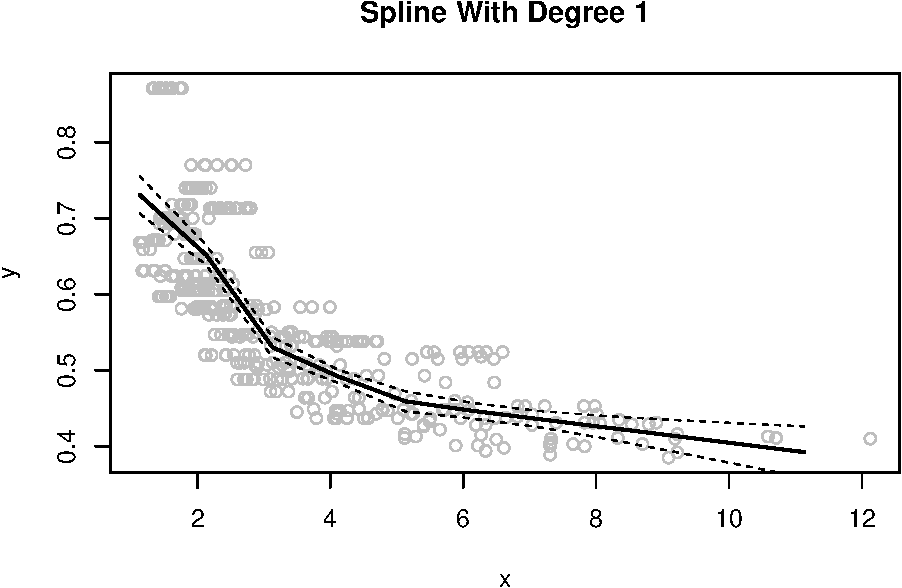
\includegraphics{hw4_files/figure-latex/unnamed-chunk-10-1.pdf}

\begin{Shaded}
\begin{Highlighting}[]
\KeywordTok{ggplot}\NormalTok{() }\OperatorTok{+}\StringTok{ }\KeywordTok{theme_bw}\NormalTok{() }\OperatorTok{+}
\StringTok{  }\KeywordTok{geom_density}\NormalTok{(}\KeywordTok{aes}\NormalTok{(}\DataTypeTok{x =}\NormalTok{ ATT[}\DecValTok{2}\NormalTok{,] }\OperatorTok{-}\StringTok{ }\KeywordTok{mean}\NormalTok{(ATT0)), }\DataTypeTok{color =} \StringTok{"maroon"}\NormalTok{) }\OperatorTok{+}\StringTok{ }\KeywordTok{labs}\NormalTok{(}\DataTypeTok{x =} \StringTok{"Lin's Estimator"}\NormalTok{)}
\end{Highlighting}
\end{Shaded}

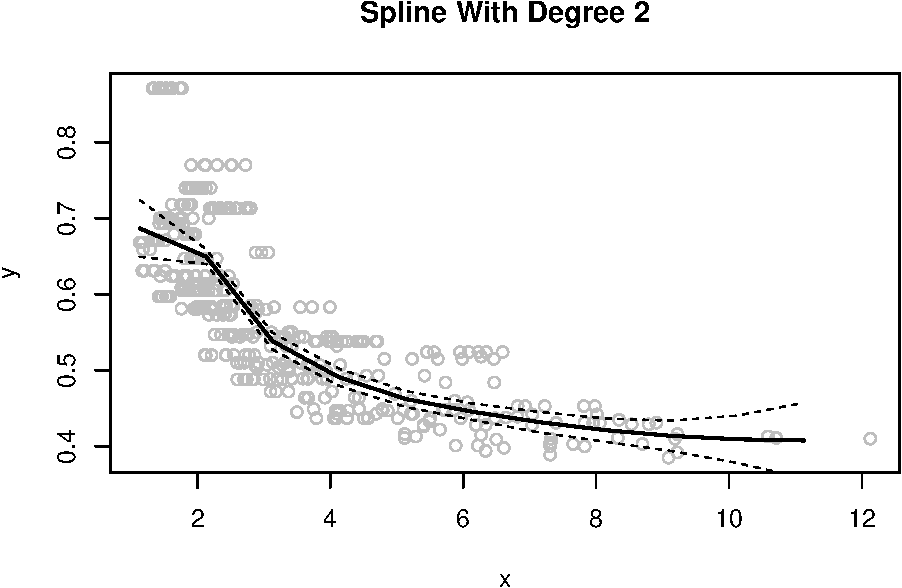
\includegraphics{hw4_files/figure-latex/unnamed-chunk-10-2.pdf}

\begin{Shaded}
\begin{Highlighting}[]
\KeywordTok{ggplot}\NormalTok{() }\OperatorTok{+}\StringTok{ }\KeywordTok{theme_bw}\NormalTok{() }\OperatorTok{+}
\StringTok{  }\KeywordTok{geom_density}\NormalTok{(}\KeywordTok{aes}\NormalTok{(}\DataTypeTok{x =}\NormalTok{ ATT[}\DecValTok{3}\NormalTok{,] }\OperatorTok{-}\StringTok{ }\KeywordTok{mean}\NormalTok{(ATT0)), }\DataTypeTok{color =} \StringTok{"maroon"}\NormalTok{) }\OperatorTok{+}\StringTok{ }\KeywordTok{labs}\NormalTok{(}\DataTypeTok{x =} \StringTok{"Hovik-Thompson"}\NormalTok{)}
\end{Highlighting}
\end{Shaded}

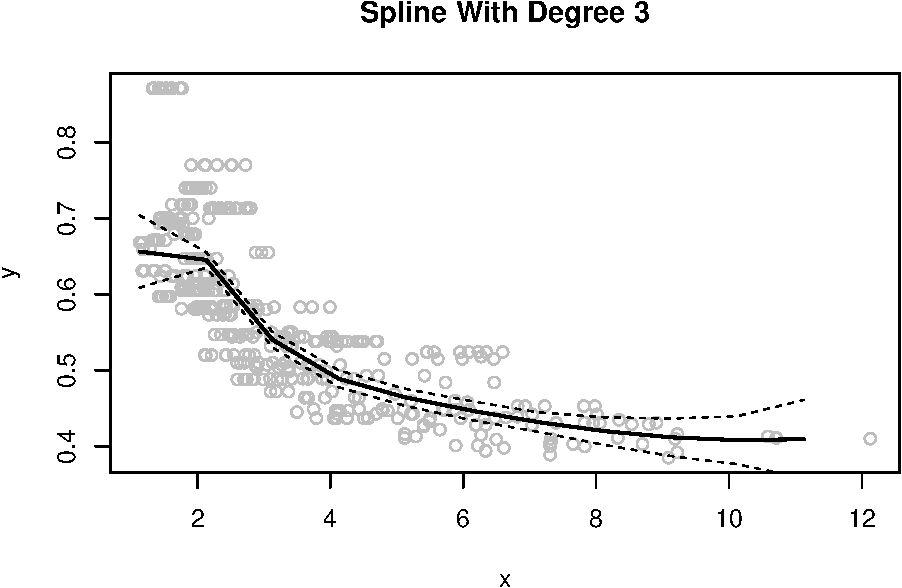
\includegraphics{hw4_files/figure-latex/unnamed-chunk-10-3.pdf}

\begin{Shaded}
\begin{Highlighting}[]
\KeywordTok{ggplot}\NormalTok{() }\OperatorTok{+}\StringTok{ }\KeywordTok{theme_bw}\NormalTok{() }\OperatorTok{+}
\StringTok{  }\KeywordTok{geom_density}\NormalTok{(}\KeywordTok{aes}\NormalTok{(}\DataTypeTok{x =}\NormalTok{ ATT[}\DecValTok{4}\NormalTok{,] }\OperatorTok{-}\StringTok{ }\KeywordTok{mean}\NormalTok{(ATT0)), }\DataTypeTok{color =} \StringTok{"maroon"}\NormalTok{) }\OperatorTok{+}\StringTok{ }\KeywordTok{labs}\NormalTok{(}\DataTypeTok{x =} \StringTok{"Hajek Estimator"}\NormalTok{)}
\end{Highlighting}
\end{Shaded}

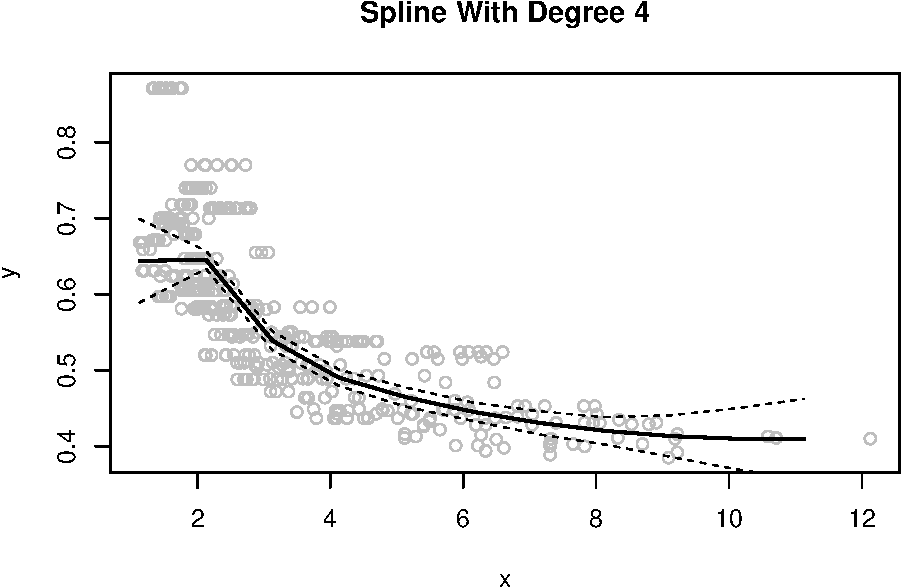
\includegraphics{hw4_files/figure-latex/unnamed-chunk-10-4.pdf}

\begin{Shaded}
\begin{Highlighting}[]
\KeywordTok{ggplot}\NormalTok{() }\OperatorTok{+}\StringTok{ }\KeywordTok{theme_bw}\NormalTok{() }\OperatorTok{+}
\StringTok{  }\KeywordTok{geom_density}\NormalTok{(}\KeywordTok{aes}\NormalTok{(}\DataTypeTok{x =}\NormalTok{ ATT[}\DecValTok{5}\NormalTok{,] }\OperatorTok{-}\StringTok{ }\KeywordTok{mean}\NormalTok{(ATT0)), }\DataTypeTok{color =} \StringTok{"maroon"}\NormalTok{) }\OperatorTok{+}\StringTok{ }\KeywordTok{labs}\NormalTok{(}\DataTypeTok{x =} \StringTok{"Doubly Robust Estimator"}\NormalTok{)}
\end{Highlighting}
\end{Shaded}

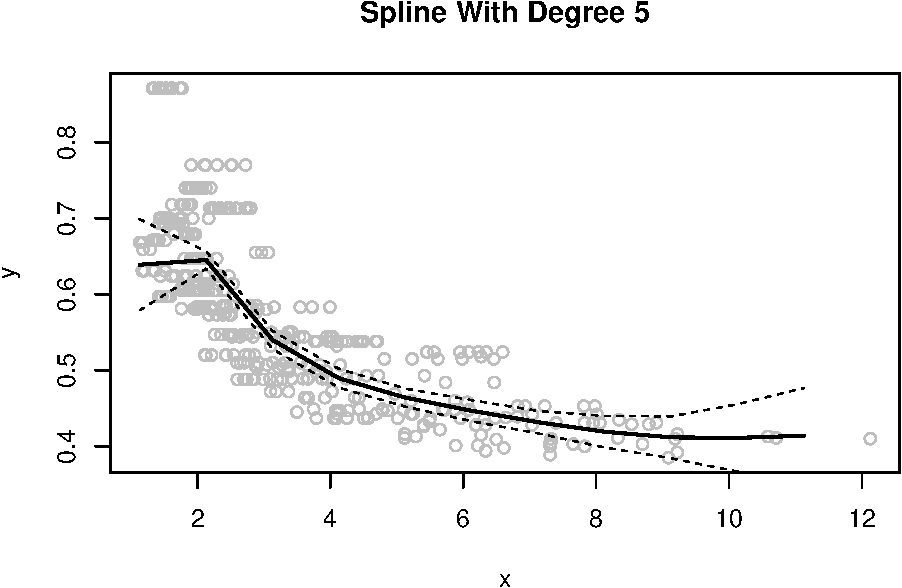
\includegraphics{hw4_files/figure-latex/unnamed-chunk-10-5.pdf}

\begin{Shaded}
\begin{Highlighting}[]
\KeywordTok{apply}\NormalTok{(ATT, }\DecValTok{1}\NormalTok{, sd)}
\end{Highlighting}
\end{Shaded}

\begin{verbatim}
## [1] 0.1895128 0.2094865 0.7741395 0.3772193 0.2608904
\end{verbatim}

\begin{Shaded}
\begin{Highlighting}[]
\KeywordTok{apply}\NormalTok{(SEboot, }\DecValTok{1}\NormalTok{, mean)}
\end{Highlighting}
\end{Shaded}

\begin{verbatim}
## [1] 0.1847593 0.2089299 0.5328994 0.3129829 0.2457885
\end{verbatim}

\begin{Shaded}
\begin{Highlighting}[]
\KeywordTok{apply}\NormalTok{(ATT, }\DecValTok{1}\NormalTok{, mean) }\OperatorTok{-}\StringTok{ }\KeywordTok{mean}\NormalTok{(ATT0) }\OperatorTok{-}\StringTok{ }\FloatTok{1.96}\OperatorTok{*}\KeywordTok{apply}\NormalTok{(ATT, }\DecValTok{1}\NormalTok{, sd)}
\end{Highlighting}
\end{Shaded}

\begin{verbatim}
## [1] -0.7351320 -0.4171376 -1.5151086 -0.7017150 -0.5218098
\end{verbatim}

\begin{Shaded}
\begin{Highlighting}[]
\NormalTok{## Case 3:}
\NormalTok{## Wrong model for both y0/ y1 and pscore}
\ControlFlowTok{for}\NormalTok{(r }\ControlFlowTok{in} \DecValTok{1}\OperatorTok{:}\NormalTok{n.sim)}
\NormalTok{\{}
\NormalTok{  x       =}\StringTok{ }\KeywordTok{matrix}\NormalTok{(}\KeywordTok{rnorm}\NormalTok{(n}\OperatorTok{*}\DecValTok{2}\NormalTok{), n, }\DecValTok{2}\NormalTok{)}
\NormalTok{  x1      =}\StringTok{ }\KeywordTok{cbind}\NormalTok{(}\DecValTok{1}\NormalTok{, x)}
\NormalTok{  beta.z  =}\StringTok{ }\KeywordTok{c}\NormalTok{(}\DecValTok{0}\NormalTok{, }\DecValTok{1}\NormalTok{, }\DecValTok{1}\NormalTok{)}
\NormalTok{  pscore  =}\StringTok{ }\DecValTok{1}\OperatorTok{/}\NormalTok{(}\DecValTok{1} \OperatorTok{+}\StringTok{ }\KeywordTok{exp}\NormalTok{(}\OperatorTok{-}\StringTok{ }\KeywordTok{as.vector}\NormalTok{(x1}\OperatorTok{\%*\%}\NormalTok{beta.z)))}
\NormalTok{  realpscore =}\StringTok{ }\DecValTok{1}\OperatorTok{/}\NormalTok{(}\DecValTok{1} \OperatorTok{+}\StringTok{ }\KeywordTok{exp}\NormalTok{(}\OperatorTok{-}\KeywordTok{as.vector}\NormalTok{(x1 }\OperatorTok{\%*\%}\StringTok{ }\KeywordTok{c}\NormalTok{(}\DecValTok{0}\NormalTok{,}\DecValTok{0}\NormalTok{,}\DecValTok{0}\NormalTok{))))}
\NormalTok{  z       =}\StringTok{ }\KeywordTok{rbinom}\NormalTok{(n, }\DecValTok{1}\NormalTok{, pscore)}
\NormalTok{  beta.y1 =}\StringTok{ }\KeywordTok{c}\NormalTok{(}\DecValTok{1}\NormalTok{, }\DecValTok{2}\NormalTok{, }\DecValTok{1}\NormalTok{)}
\NormalTok{  beta.y0 =}\StringTok{ }\KeywordTok{c}\NormalTok{(}\DecValTok{1}\NormalTok{, }\DecValTok{1}\NormalTok{, }\DecValTok{1}\NormalTok{)}
\NormalTok{  realbeta.y1 =}\StringTok{ }\KeywordTok{c}\NormalTok{(}\DecValTok{2}\NormalTok{, }\DecValTok{3}\NormalTok{, }\DecValTok{4}\NormalTok{)}
\NormalTok{  realbeta.y0 =}\StringTok{ }\KeywordTok{c}\NormalTok{(}\DecValTok{100}\NormalTok{, }\DecValTok{101}\NormalTok{, }\DecValTok{102}\NormalTok{)}
\NormalTok{  y1      =}\StringTok{ }\KeywordTok{rnorm}\NormalTok{(n, x1}\OperatorTok{\%*\%}\NormalTok{realbeta.y1)}
\NormalTok{  y0      =}\StringTok{ }\KeywordTok{rnorm}\NormalTok{(n, x1}\OperatorTok{\%*\%}\NormalTok{realbeta.y0)}
\NormalTok{  y       =}\StringTok{ }\NormalTok{z}\OperatorTok{*}\NormalTok{y1 }\OperatorTok{+}\StringTok{ }\NormalTok{(}\DecValTok{1} \OperatorTok{-}\StringTok{ }\NormalTok{z)}\OperatorTok{*}\NormalTok{y0}
\NormalTok{  ATT0[r] =}\StringTok{ }\KeywordTok{mean}\NormalTok{(y1[z}\OperatorTok{==}\DecValTok{1}\NormalTok{]) }\OperatorTok{-}\StringTok{ }\KeywordTok{mean}\NormalTok{(y0[z}\OperatorTok{==}\DecValTok{1}\NormalTok{])}
  
\NormalTok{  causaleffect =}\StringTok{ }\KeywordTok{ObsCausal.ATT}\NormalTok{(z, y, x)}
\NormalTok{  ATT[, r]     =}\StringTok{ }\NormalTok{causaleffect[}\DecValTok{1}\NormalTok{, ]}
\NormalTok{  SEboot[, r]  =}\StringTok{ }\NormalTok{causaleffect[}\DecValTok{2}\NormalTok{, ]}
\NormalTok{\}}

\KeywordTok{apply}\NormalTok{(ATT, }\DecValTok{1}\NormalTok{, mean) }\OperatorTok{-}\StringTok{ }\KeywordTok{mean}\NormalTok{(ATT0)}
\end{Highlighting}
\end{Shaded}

\begin{verbatim}
## [1] 71.292947086 -0.004852229  3.120162985  5.626615117 -0.004806452
\end{verbatim}

\begin{Shaded}
\begin{Highlighting}[]
\KeywordTok{apply}\NormalTok{(ATT, }\DecValTok{1}\NormalTok{, sd)}
\end{Highlighting}
\end{Shaded}

\begin{verbatim}
## [1] 12.08423 12.13165 61.82708 30.81661 12.13796
\end{verbatim}

\begin{Shaded}
\begin{Highlighting}[]
\KeywordTok{apply}\NormalTok{(SEboot, }\DecValTok{1}\NormalTok{, mean)}
\end{Highlighting}
\end{Shaded}

\begin{verbatim}
## [1] 11.91909 11.84323 45.62230 22.54042 11.84496
\end{verbatim}


\end{document}
